\section{Problem Set 9}
\subsection{Catching Up}
The main issues that needed to be addressed in the previous problem sets were the inaccuracy of the geometric linear mapping in PS3, improving the impulsive control to use the semi-analytical closed-form solutions from \cite{chernick2018new} in PS5, fixing the delta-v usage calculation of the continuous control in PS6, and incorporating updates from PS7 and PS8 into PS9. Along with these major fixes, each problem set was also updated with minor fixes for readability and accuracy.
\begin{enumerate}
    \item For problem set 1, we clarified which ROEs are being used when throughout the project. Specifically, the ROES from the NASA Starling mission are used in problem sets 1 and 2 to investigate and verify the dynamics models. For later problem sets, our custom ROEs are used to simulate rendezvous and docking, except for problem set 4 where the prescribed ROEs are used.
    \item For problem set 2, we consolidated some repeated equations, updated the RTN projection plot for readability, added a new RTN projection plot to showcase the effects of the maneuver, and added supportive analysis.
    \item For problem set 3, we updated the ROEs to match those chosen in later problem sets, fixed geometric linear mapping so that it is more accurate than the Yamanaka-Ankersen solution, created more readable figures to highlight the differences between the methods, and  improved overall readability through spelling and grammar fixes.
    \item For problem set 4, we included clarification over the usage of given ROEs versus custom ROEs, and improved the language and reasoning about drifts observed in $\delta \lambda$.
    \item For problem set 5, major changes were made to the way we do impulsive control. Previously, only a naive-least squares with a prescribed set of maneuver locations was used to achieve the desired control. This was much more inefficient, and led to thrust directions in arbitrary directions. A lot of this was improved to use more optimal closed-form semi-analytical solutions for in-plane and out-of-plane control taken from \cite{damicothesis} and \cite{chernick2018new}. Station-keeping was also updated to work alongside the large maneuvers between modes in the simulation. The problem set 5 section write-up has been updated to include the methodology used for the closed-form control solutions and the improved results.
    \item For problem set 6, we added a missing negative sign in the equation for drift in $\delta \lambda$, and fixed the calculation and plotting of delta-v's for Lyapunov control so that they are much more reasonable and closer to delta-v lower bound 
    \item For problem set 7, we incorporated improvements into problem set 8 since it was the implementation of the EKF outlined in problem set 7. The major update was that we no longer estimate the absolute chief state in our EKF. This was done to simplify the measurement model and the EKF mean propagation. 
    \item For problem set 8, we incorporated all remaining improvements into problem set 9. The main improvements include the addition of drag into our ground truth force model, better justification of noise values, and the addition of the 3-sigma region to the EKF plots. These were along with the successful integration of navigation and control and the addition of some bonus material. 
\end{enumerate}


\subsection{Integration of Navigation and Control}
\subsubsection{Inclusion of Drag Perturbations in Ground Truth}
From problem set 8, the ground truth and EKF implementations were improved. First, drag force was introduced into the force model of the ground truth to distinguish it further from the EKF mean ROE propagation via STMs. The ground truth now propagates the absolute orbital elements of the chief and deputy spacecraft with GVEs that include secular J2 and drag effects. The secular J2 effects have been described previously in Section \ref{sec:osc_mean_J2}. The atmospheric drag force is modeled as: 

\begin{equation}
    D = \frac{1}{2} \, \rho \, v^2 \, C_D \, A
\end{equation}

where $\rho$ is the atmospheric density [kg/m$^3$], $v$ is the spacecraft’s velocity relative to the atmosphere [km/s], $C_D$ is the drag coefficient [–], $A$ is the cross-sectional area of the spacecraft [m$^2$].

The drag coefficient, $C_D$, is assumed to be 2.2, which approximates the satellite as a flat plate and is a conservative assumption. The cross-sectional area and mass of the spacecraft are based on standard values for 6U cubesats, since the NASA Starling satellites are built on a 6U Blue Canyon XB1 bus. \cite{miller2024starling} The standard dimensions of a 6U cubesat are 20 by 10 by 34 cm and the standard mass is about 12 kg. \cite{cubesatSpec} Therefore, to be conservative, the cross-sectional area is approximated as 0.20 $m$ by 0.34 $m$ or 0.068 $m^2$. The spacecraft's velocity relative to the atmosphere is approximated as its velocity in ECI, assuming the atmosphere is not moving. To find the atmospheric density at a given altitude, a simple atmosphere model is used based on Vallado Table 8-4, as shown below.\cite{book:Vallado}

\begin{table}[H]
\centering
\begin{tabular}{|c|c|}
\hline
\textbf{Altitude (km)} & \textbf{Density $\rho$ (kg/m$^3$)} \\
\hline
150  & $2.070 \times 10^{-9}$ \\
200  & $2.789 \times 10^{-10}$ \\
250  & $7.248 \times 10^{-11}$ \\
300  & $2.418 \times 10^{-11}$ \\
350  & $9.518 \times 10^{-12}$ \\
400  & $3.725 \times 10^{-12}$ \\
450  & $1.585 \times 10^{-12}$ \\
500  & $6.967 \times 10^{-13}$ \\
600  & $1.454 \times 10^{-13}$ \\
700  & $3.614 \times 10^{-14}$ \\
800  & $1.170 \times 10^{-14}$ \\
900  & $5.245 \times 10^{-15}$ \\
1000 & $3.019 \times 10^{-15}$ \\
\hline
\end{tabular}
\caption{Atmospheric density vs. altitude (example values)}
\label{tab:atmospheric_density}
\end{table}

The corresponding perturbing acceleration due to atmospheric drag is:

\begin{equation}
    a_{\text{drag}} = \frac{D}{m} = \frac{1}{2} \cdot \frac{\rho \, v^2 \, C_D \, A}{m}
\end{equation}

In the Radial-Tangential-Normal (RTN) frame, drag is assumed to only act in the tangential direction (opposite the velocity vector), so the perturbing acceleration components become:

\begin{equation}
    \begin{aligned}
        f_R &= 0 \\
        f_T &= -a_{\text{drag}}^{(\text{km/s}^2)} \\
        f_N &= 0
    \end{aligned}
\end{equation}

Thus, the full perturbing acceleration vector in the RTN frame is:

\begin{equation}
    \vec{f}_{\text{drag}}^{RTN} =
    \begin{bmatrix}
        0 \\
        -\frac{1}{2} \cdot \frac{\rho \, v^2 \, C_D \, A}{m} \\
        0
    \end{bmatrix}
    \quad \text{[km/s$^2$]}
\end{equation}

This perturbing acceleration is then plugged into the GVEs for near-circular orbits along with the J2 effects to ultimately determine the impact of drag and J2 on the absolute orbital elements. 

\begin{align*}
\frac{da}{dt} &= \frac{2}{n} \, f_T \\
\frac{d e_x}{dt} &= \frac{1}{n a} \left( \sin(u) \, f_R + 2 \cos(u) \, f_T \right) \\
\frac{d e_y}{dt} &= \frac{1}{n a} \left( -\cos(u) \, f_R + 2 \sin(u) \, f_T \right) \\
\frac{di}{dt} &= \frac{1}{n a} \cos(u) \, f_N \\
\frac{d\Omega}{dt} &= \frac{1}{n a \sin(i)} \sin(u) \, f_N \\
\frac{du}{dt} &= \mathrm{rad2deg} \left( \frac{1}{n a} \left( -2 f_R - \sin(u) \cot(i) f_N \right) \right)
\end{align*}

The implementation of drag was verified by observing a secular decay in the absolute orbital elements of all the spacecraft. The inclusion of drag in the ground truth force model ensures further differentiates it from the EKF mean propagation which uses an STM to propagate ROEs. However, since all spacecraft are experiencing similar drag in their absolute frames, there is not a significant effect on their relative motion. Thus, even though the EKF does not include drag force, it still tracks well, as will be discussed later. 

\subsubsection{Measurement Noise Improvements}
Second, the injected measurement noise was improved to better reflect realistic noisy measurements. For absolute measurements, we assume that we receive ECI measurements of the two deputy spacecraft through GPS. According to literature, real-time space-borne GPS accuracy for LEO satellites has a baseline of 10 meters. With the addition of carrier-phase signal and/or dynamic orbit determination, this accuracy can get down to 1 meter and lower. \cite{montenbruck2008precision} We make a conservative assumption of 10-meter noise in our ECI measurements. 

For relative measurements, there are a wide range of sensors that provide varying levels of accuracy. One approach of using GPS, crosslink (which is a radio link between spacecraft that is used to transfer data and also measure range), and celestial object measurements yields a relative navigation RMS error of 10 cm. \cite{long2002relative} At closer ranges, such as in the docking phase, LiDAR can be used, which can achieve an accuracy of 1 to 3 cm. \cite{cail_software_usu} We make a conservative assumption of 0.1-meter noise in our RTN measurements. 

Thus, the added noise $V_t$ for a single deputy is given by:

\begin{align}
    V_{t} = \mathcal{N}\left(0, \begin{bmatrix}
        0.0001 I_3 \\
         0.01I_3 \\
 \end{bmatrix}\right) km \label{eq:added_noise_new}
\end{align}

Note that this noise is in kilometers, since the ECI and RTN values are in kilometers. Also, our measurement vector is made up of RTN measurements stacked on top of ECI measurements. 

\subsubsection{Simulation and Control Architecture}
For this pset, we are integrating our navigation and control mechanisms. As such, in our simulation loop, we are:
\begin{itemize}
    \item Propagate the ground truth states for SV1, SV2, and SV3. Here, we choose to represent the states of our satellites in absolute, quasi-nonsingular orbital elements, and propagate them using the Gauss Variational Equations (GVEs) with J2 and drag effects. 
    \item Plan maneuvers. Here, the team decided to use a combination of both impulsive and continuous control methods. Impulsive maneuvers (semi-analytical closed-form methods) were used for the large orbit reconfigurations. This is where a large, high-thrust low-ISP thruster like a chemical rocket engine could be used. Continuous control (Lyapunov-based control) was used for station keeping and reducing any drift left from the impulse maneuvers. In implementation, this is where low-thrust high-Isp thrusters such as Hall-effect thrusters could be used. Also, continuous control is used due to the minimum impulse bit requirements likely being smaller than what chemical propulsion could provide. The estimates of the deputy states were used in planning and control.
    \item Apply the control action. This is applied as a $\Delta v$ to the state. As discussed in the bonus section, some noise was added to the actuator as another source of application uncertainty.
    \item Generate measurements based on the measurement model previously discussed, and the ground truth values from SV1, SV2, SV3.
    \item Use the measurements and prior states to generate an estimate of SV2 and SV3's ROEs using our Extended Kalman Filter implementation. These estimates are then used for planning.
\end{itemize}

The full order of operations was critical to ensure that the correct values for the ground truth and the estimates were used for planning, so as to prevent any control or estimation instabilities due to a time delay. This is shown in detail in Figure \ref{fig:nav_control_arch}.

\begin{figure}[H]
    \centering
    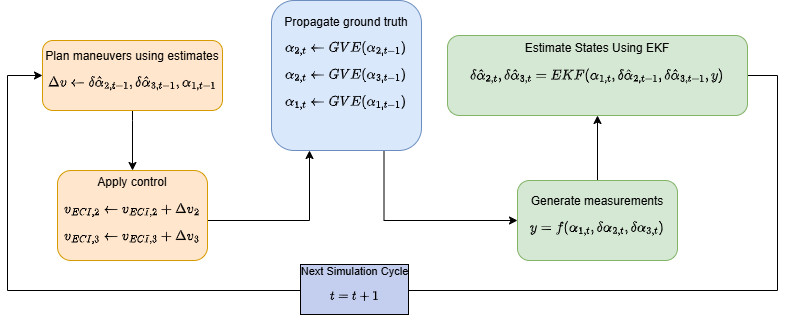
\includegraphics[width=0.85\linewidth]{LaTeX/PS9/soss_control_nav_arch.png}
    \caption{The complete control, simulation, and navigation architecture}
    \label{fig:nav_control_arch}
\end{figure}

\subsubsection{Results and Analysis}
With the control implemented as discussed above (a combination of PS5 and PS6 methods), and an Extended Kalman Filter implemented as in PS8, we get the results shown in 

\textbf{\textit{Control Performance}}

First, we look at the performance of the combination of impulsive and continuous control in how well it tracks our desired state. In Figure \ref{fig:roe_error_control_sv2}, we see that the continuous control station-keeping doesn't fully converge all the ROE errors to $0$, but keeps the error bounded. ROEs $\delta e_x$ and $\delta i_y$ noticeably converge to a non-zero steady state, but this is deemed as acceptable error, as it remains within the meter-level accuracy requirements expected for SV2's position.

\begin{figure}[H]
    \centering
    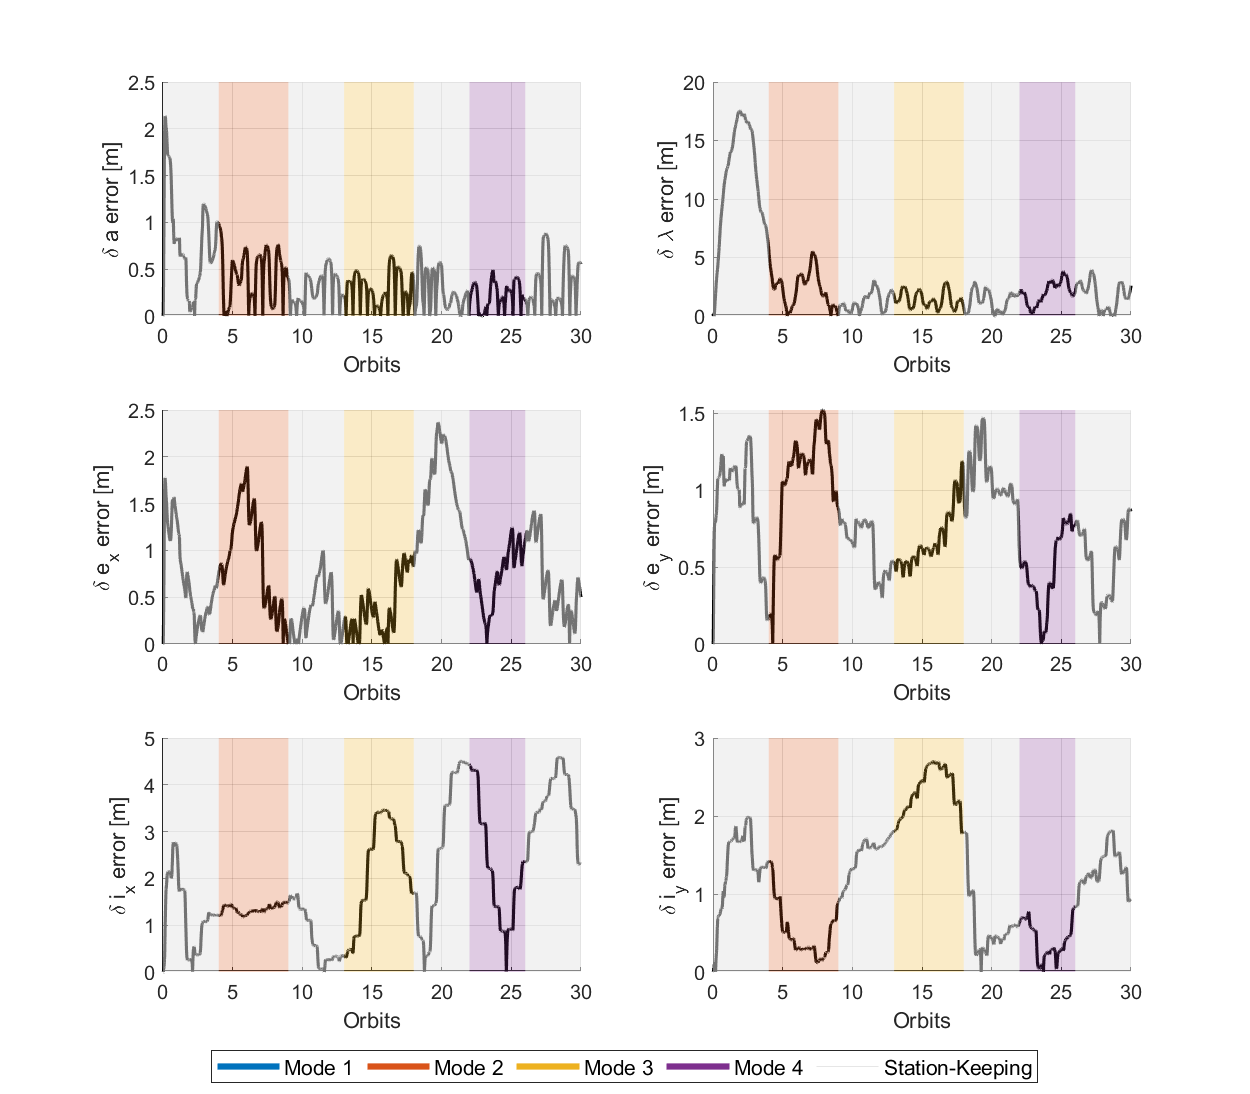
\includegraphics[width=0.7\linewidth]{sim/figures/PS9/ROE_error_over_time_modes_SV2.png}
    \caption{Error between the true ROEs and the desired ROEs for SV2}
    \label{fig:roe_error_control_sv2}
\end{figure}

In Figures \ref{fig:roe_error_control_sv3} and \ref{fig:roe_final_SV3_planes}, we see that all our ROE states converge to their desired values with the impulsive maneuvers. $\delta a$ and $\delta \lambda$ become non-zero during these maneuvers, but are controlled back to their desired states. $\delta e_x$ and $\delta i_x$ are not explicitly controlled, and are affected by slight offsets in maneuver times and J2 effects.
\begin{figure}[H]
    \centering
    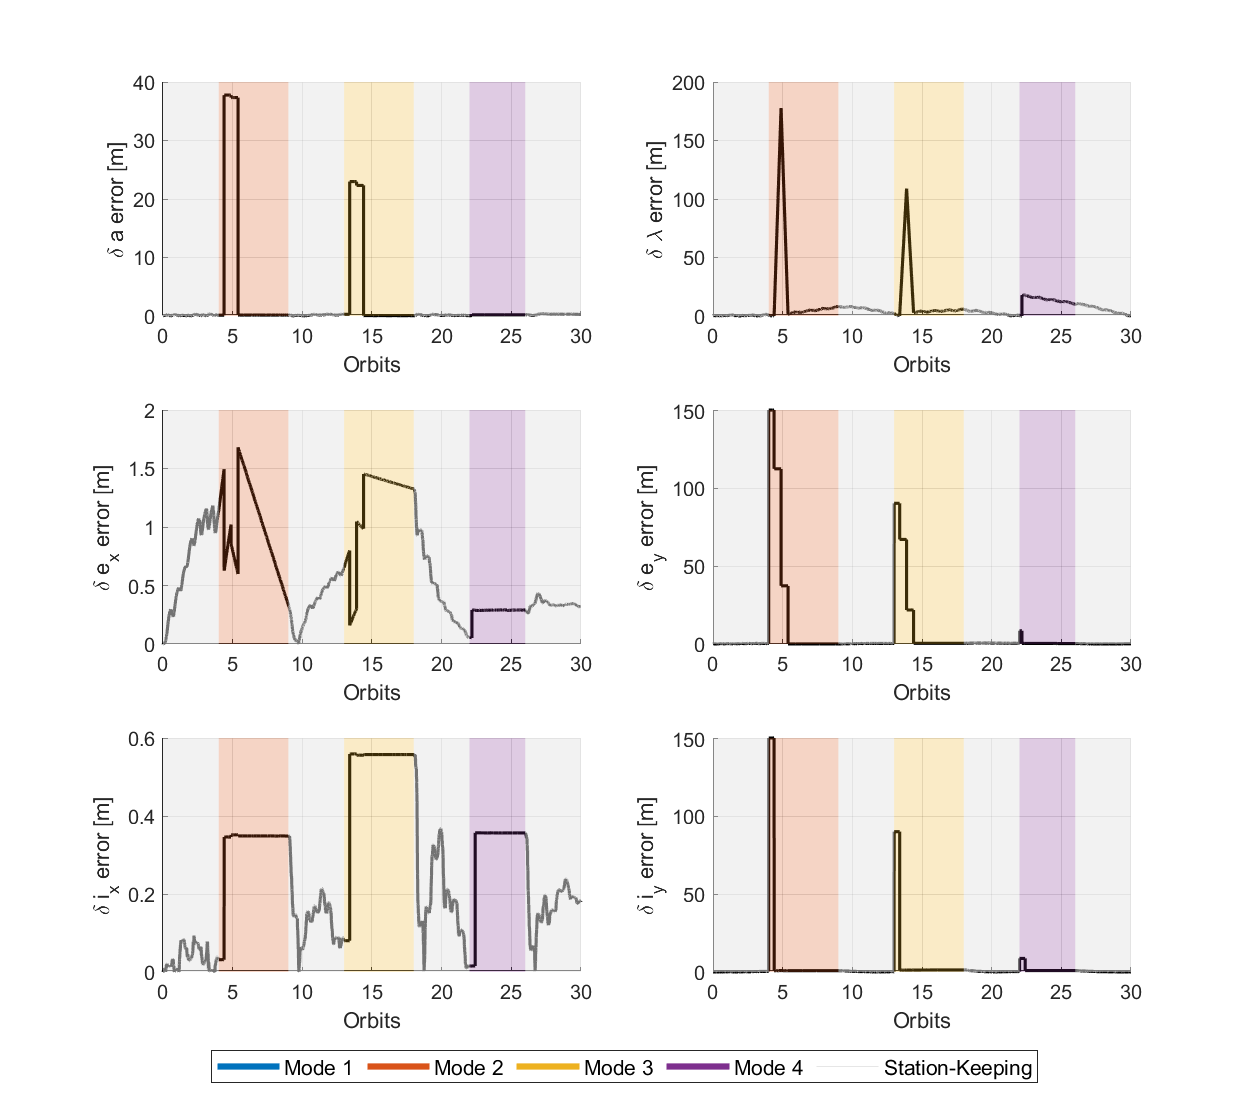
\includegraphics[width=0.7\linewidth]{sim/figures/PS9/ROE_error_over_time_modes_SV3.png}
    \caption{Error between the true ROEs and the desired ROEs for SV3}
    \label{fig:roe_error_control_sv3}
\end{figure}

\begin{figure}[H]
    \centering
    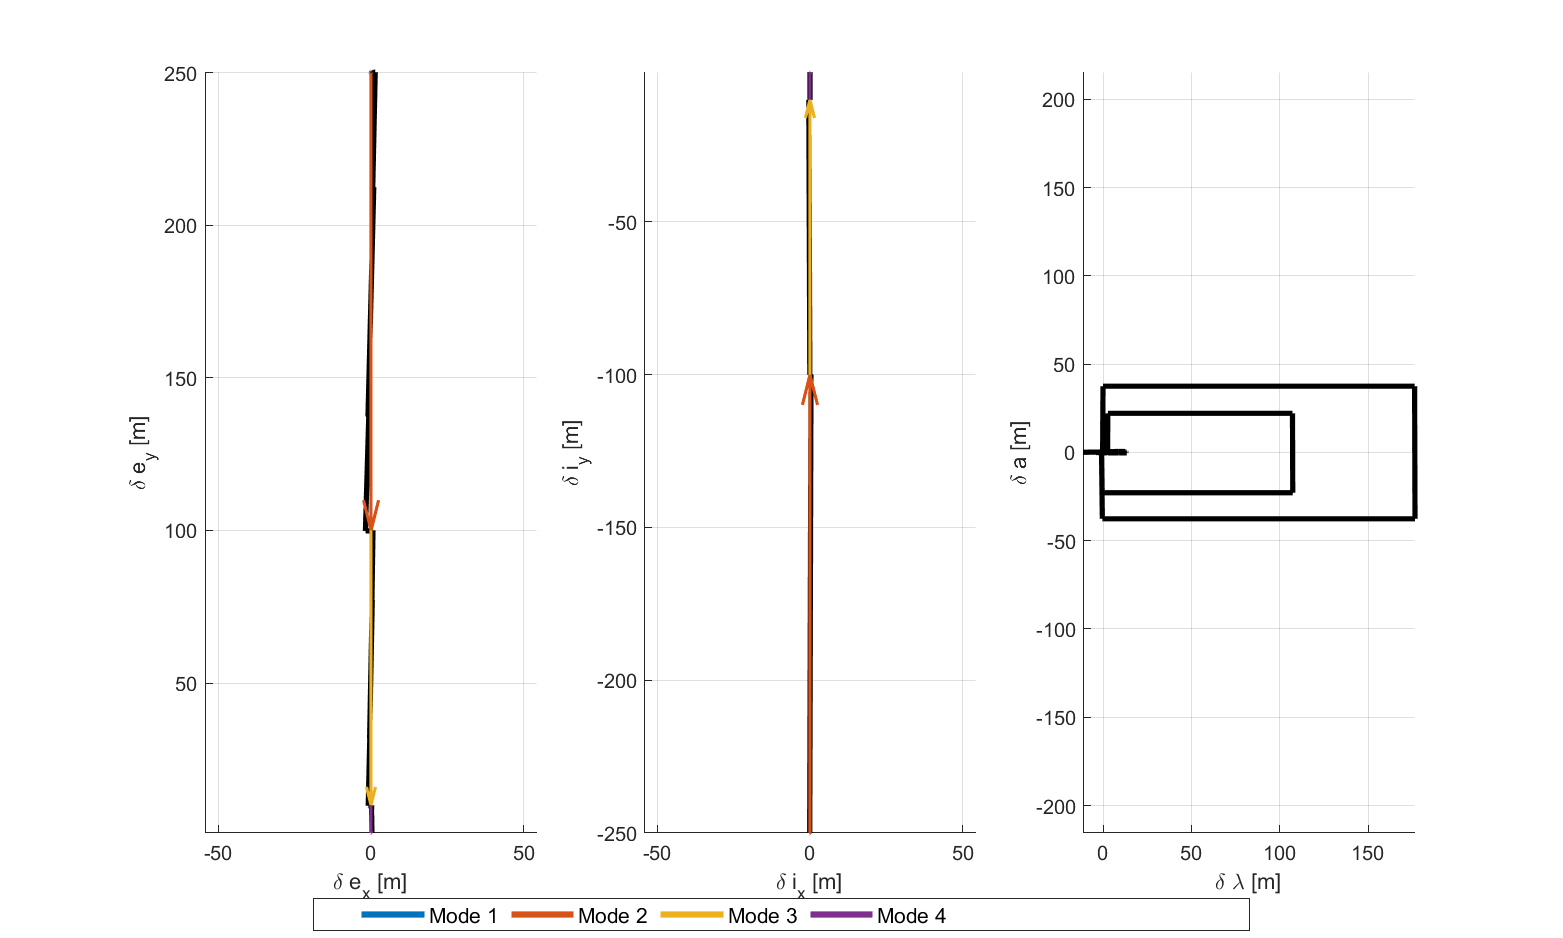
\includegraphics[width=0.7\linewidth]{sim/figures/PS9/ROE_planes_modes_SV3.png}
    \caption{ROEs of SV3 in different ROE planes}
    \label{fig:roe_final_SV3_planes}
\end{figure}

Figures \ref{fig:delta_v_cumulative_sv2} and \ref{fig:delta_v_cumulative_sv3} showcase the $\Delta v$ over time for SV2 and SV3.  
\begin{figure}[H]
    \centering
    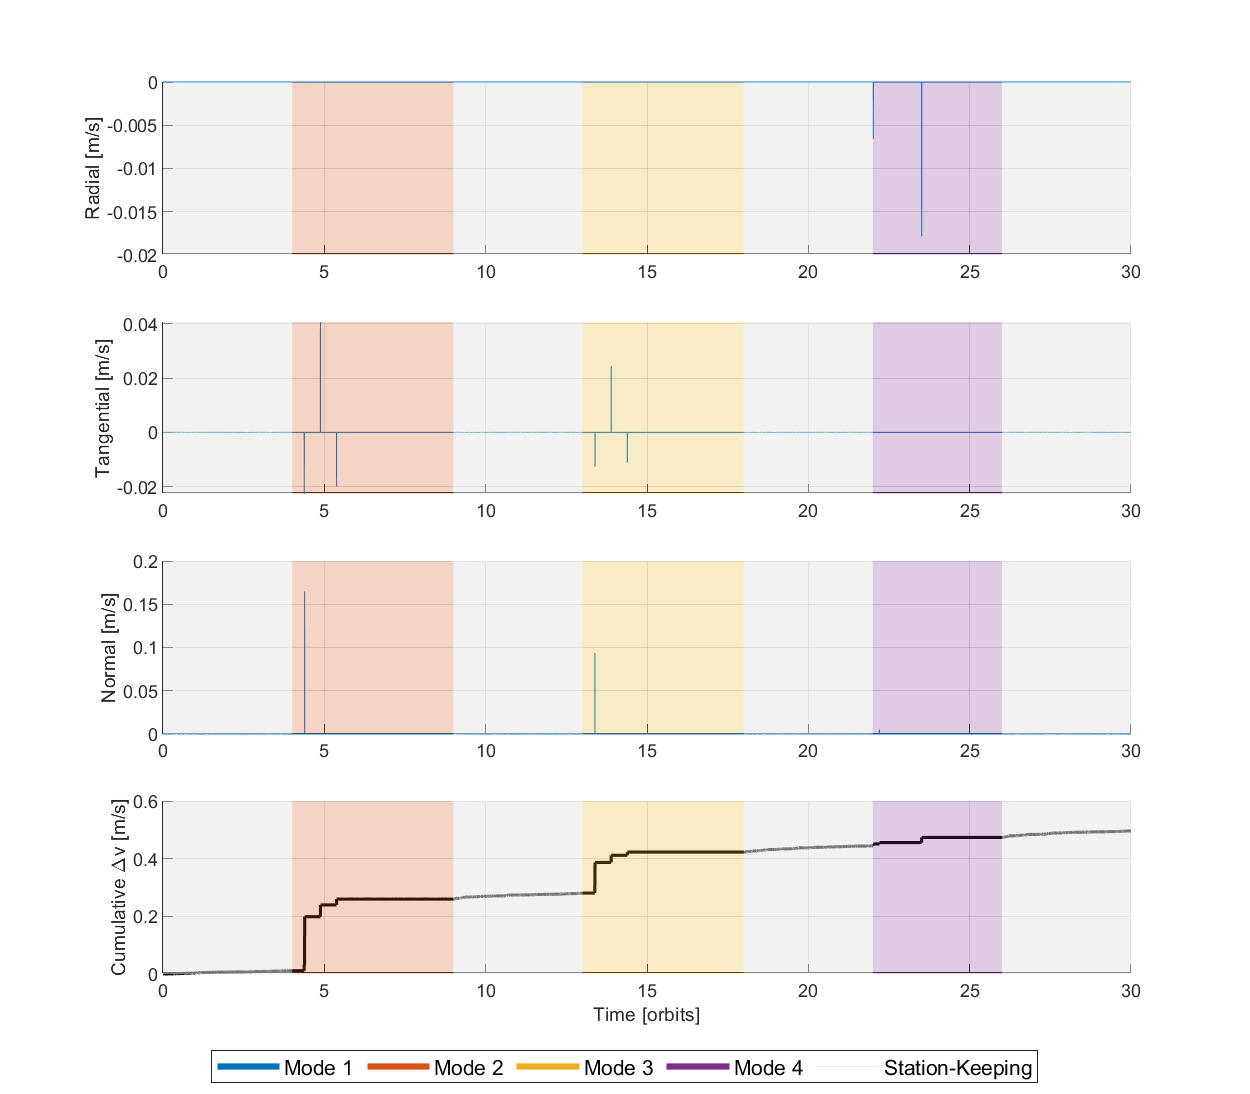
\includegraphics[width=0.7\linewidth]{sim/figures/PS9/delta_v_cumulative_timeline_modes_SV3.png}
    \caption{$\Delta v$ over time for SV3. Note that this uses impulsive control for the maneuvers, but continuous control for station keeping.}
    \label{fig:delta_v_cumulative_sv3}
\end{figure}

\begin{figure}[H]
    \centering
    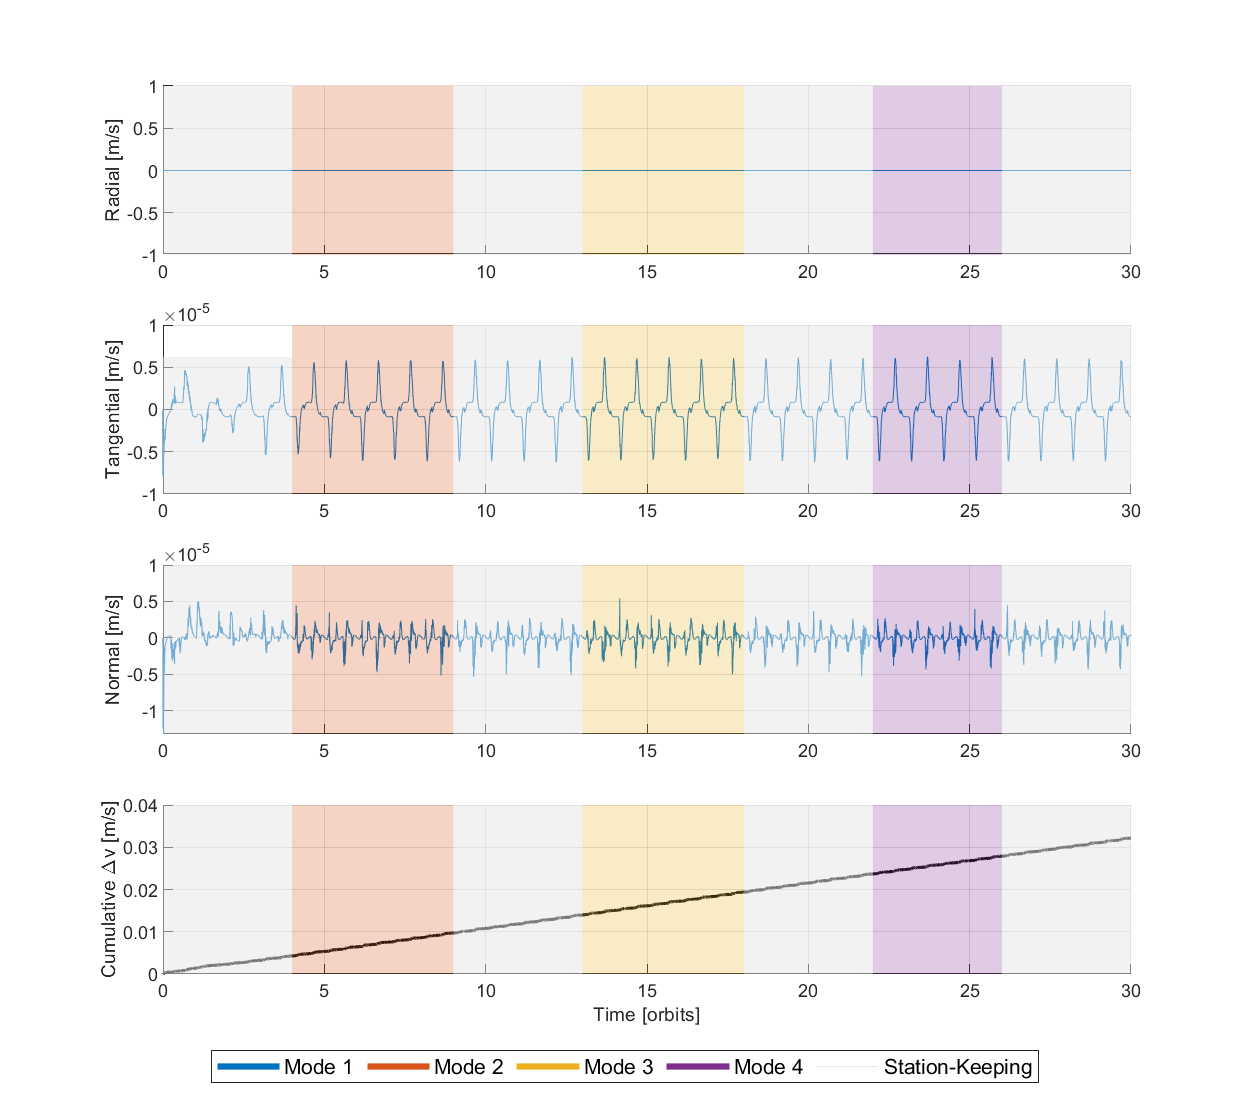
\includegraphics[width=0.7\linewidth]{sim/figures/PS9/delta_v_cumulative_timeline_modes_SV2.png}
    \caption{$\Delta v$ over time for SV2. This only uses continuous control for station keeping.}
    \label{fig:delta_v_cumulative_sv2}
\end{figure}

\textbf{\textit{Navigation Performance}}

Now, we look specifically at comparisons between the true states and the estimate states. Figures \ref{fig:sv2_ekf_comparison_ps9} and \ref{fig:sv3_ekf_comparison_ps9} show the true state and the EKF estimated states over time, along with the covariance bounds over this time. We see that SV2's estimation works well, with small covariance bounds and good tracking. SV3 has some interesting behavior. Specifically, because of a lower reliance on the dynamics (larger process noise $Q$), the covariance bounds are significantly larger. In addition, during the impulses, we see large difference in error between the estimated states and true states. This is easy to see in Figure \ref{fig:ekf_error_ps9_sv3}. Although we are accounting for the control input in our EKF, it is unable to predict the behavior during these impulses, incorrectly estimating a spike in $\delta e_x$ and $\delta i_x$ when there is no such spike in the true values. Relying more on the process step reduces these spikes, but makes the response to the spike too slow for some of the fast changes in. Experiments with putting a lower process noise on $\delta e_x$ and $\delta i_x$ yieled mixed results (including loss of control due to poor estimates resulting in poor planning), but further tuning to the EKF may improve these results. Regardless, the estimates converge to values within acceptable error bounds.

\begin{figure}[H]
    \centering
    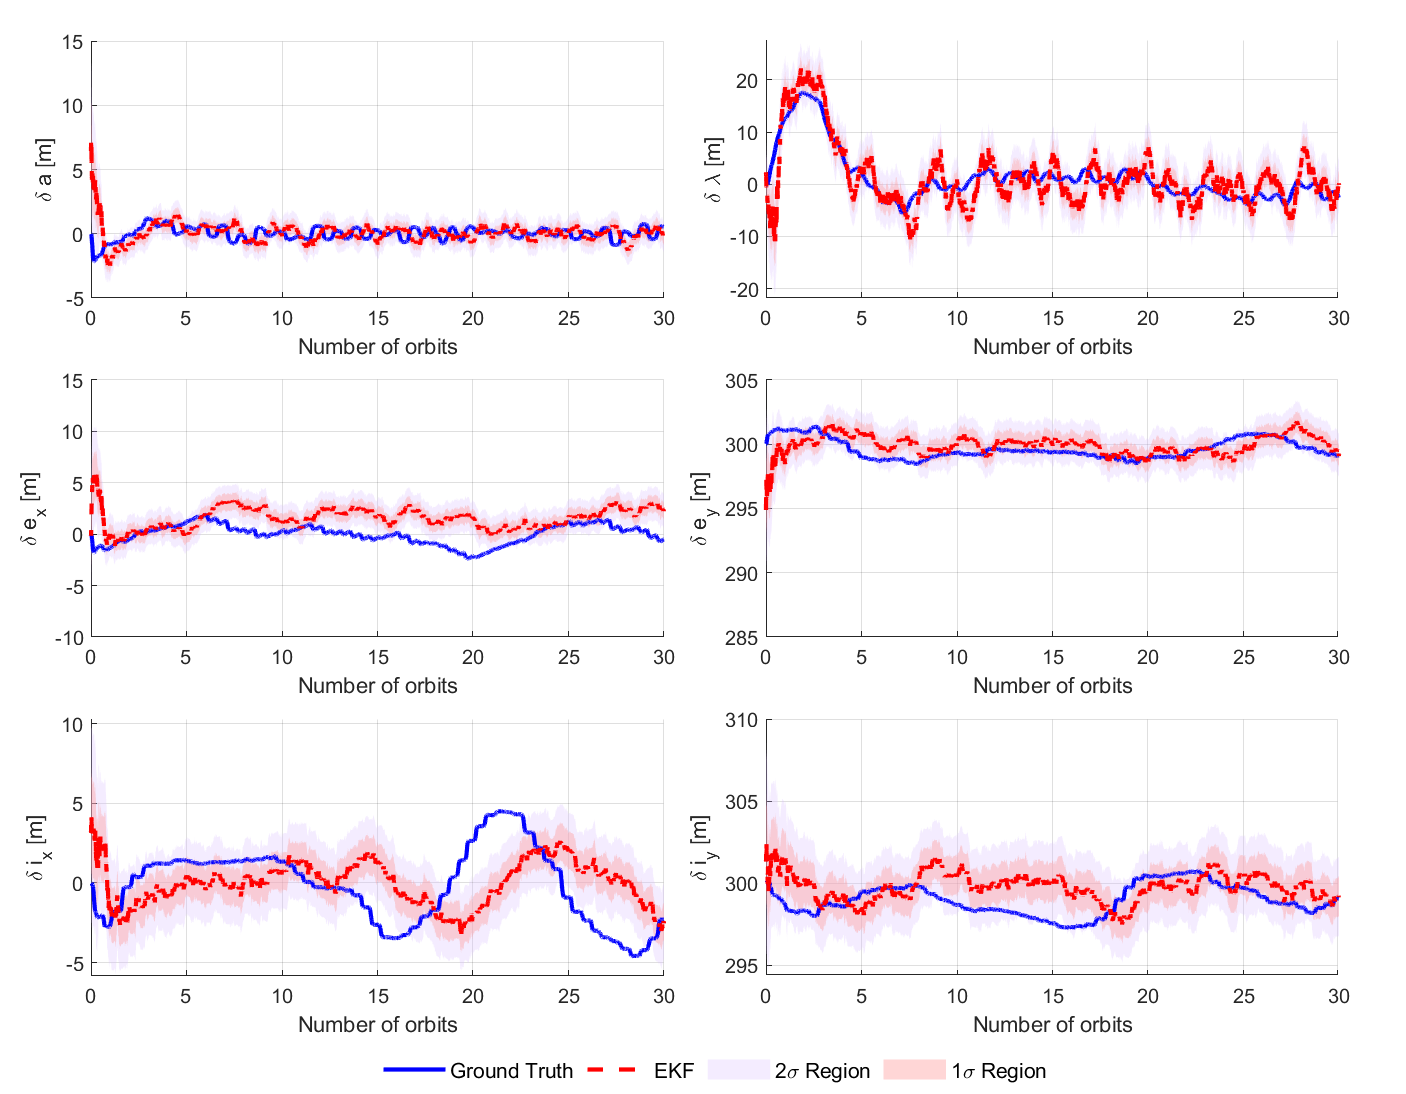
\includegraphics[width=0.7\linewidth]{sim/figures/PS9/ROE_over_time_SV2_comparison.png}
    \caption{True ROEs, estimate ROEs, and covariance bounds for SV2 over time.}
    \label{fig:sv2_ekf_comparison_ps9}
\end{figure}

\begin{figure}[H]
    \centering
    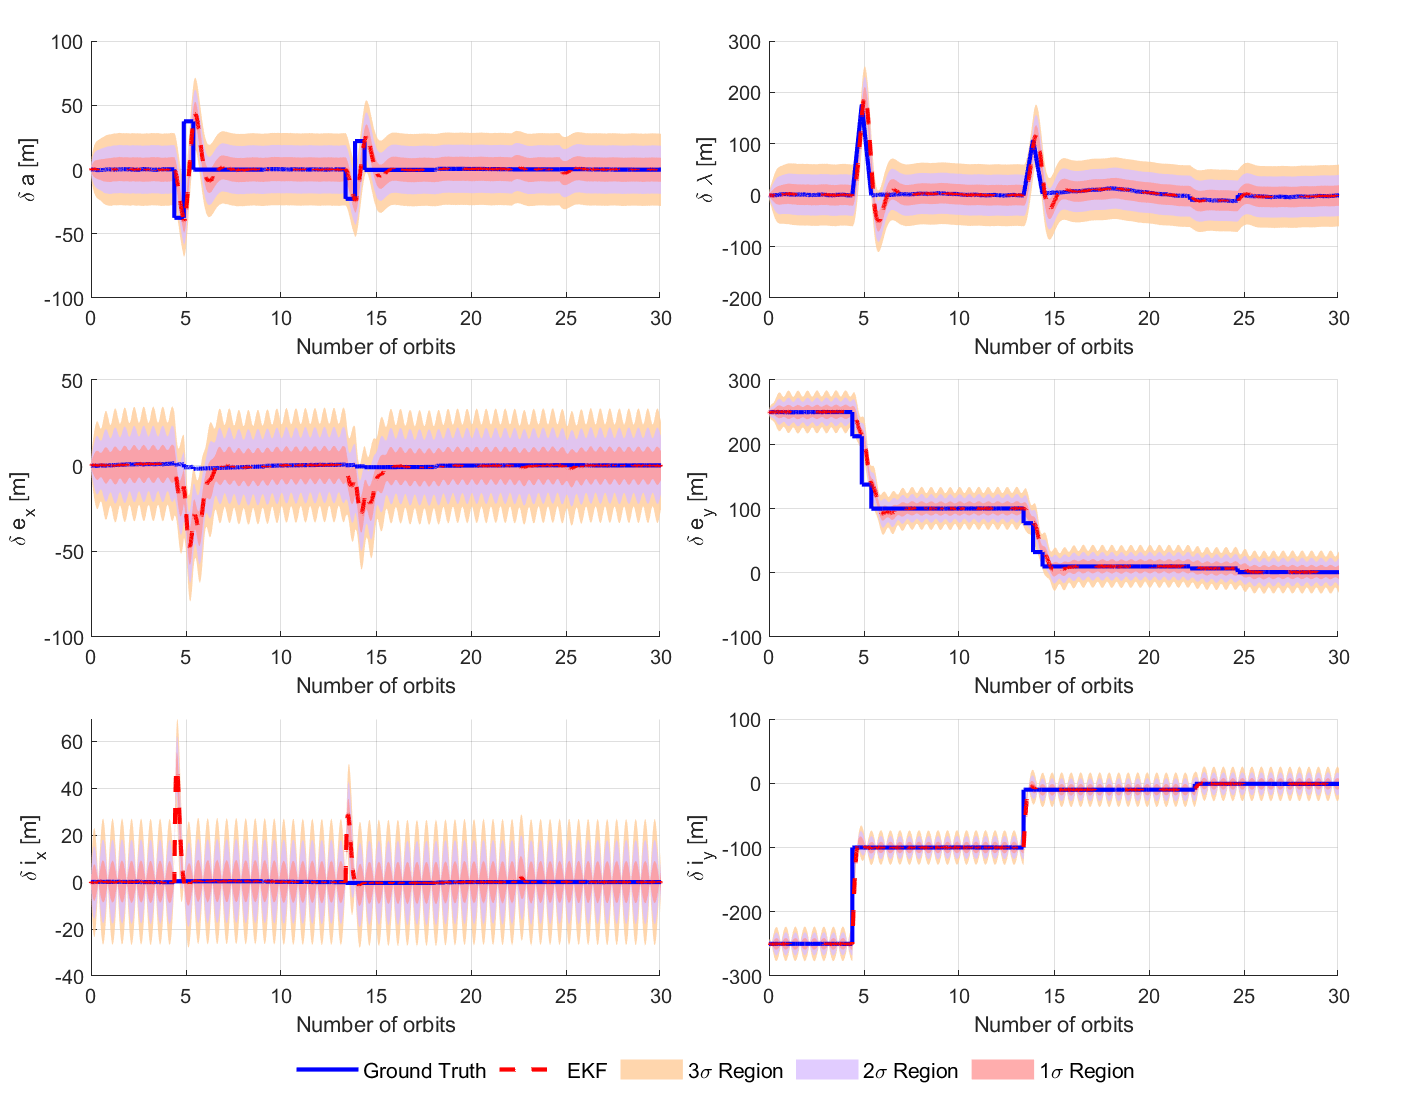
\includegraphics[width=0.7\linewidth]{sim/figures/PS9/ROE_over_time_SV3_comparison.png}
    \caption{True ROEs, estimate ROEs, and covariance bounds for SV3 over time.}
    \label{fig:sv3_ekf_comparison_ps9}
\end{figure}

\begin{figure}[H]
    \centering
    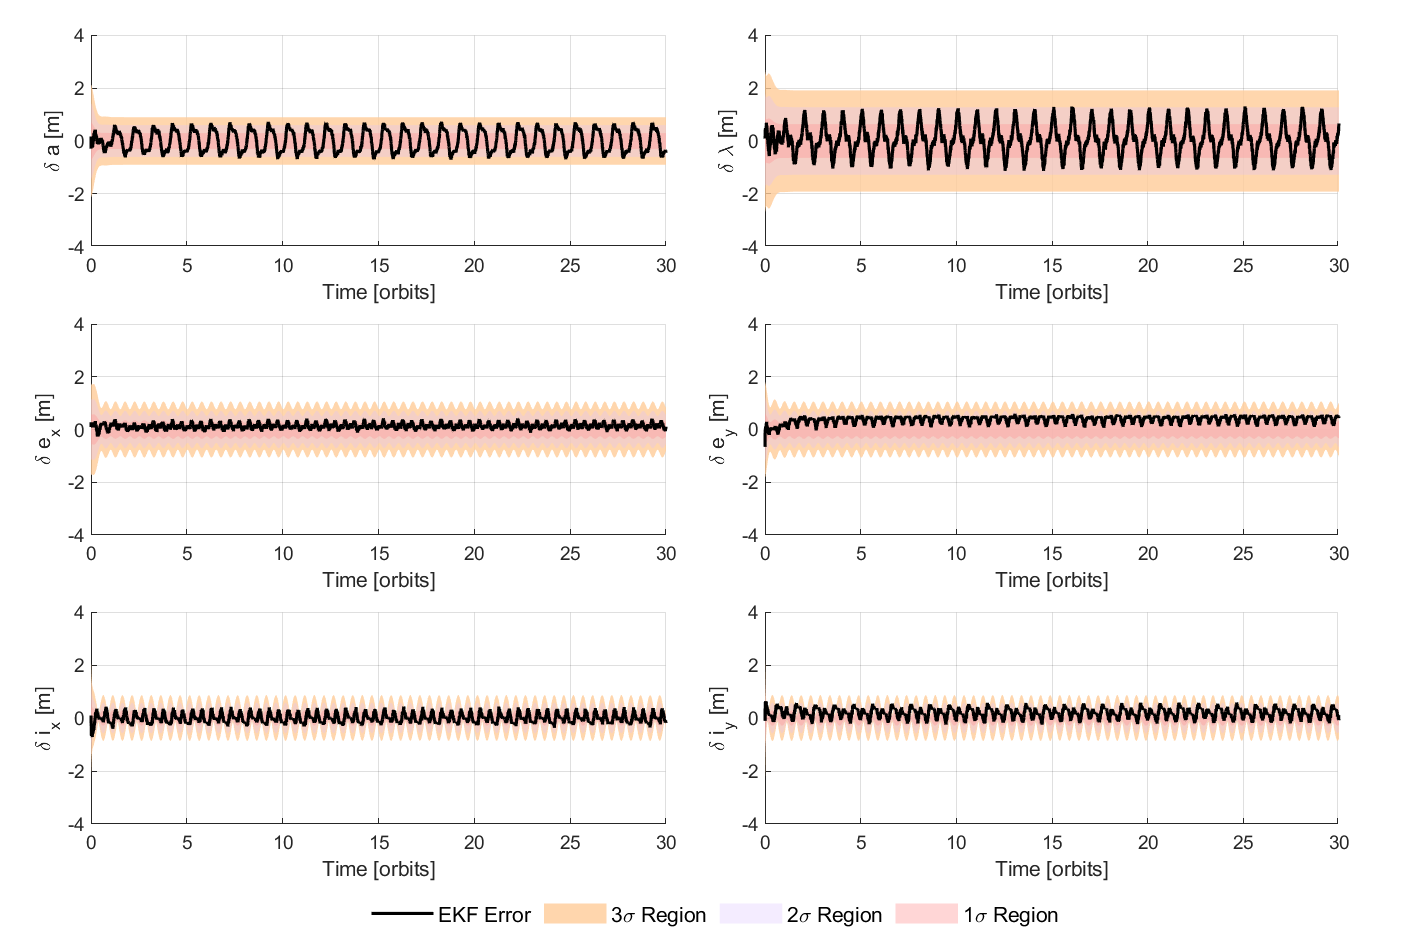
\includegraphics[width=0.7\linewidth]{sim/figures/PS9/EKF_error_SV2.png}
    \caption{SV2 EKF error over time.}
    \label{fig:ekf_error_ps9_sv2}
\end{figure}


\begin{figure}[H]
    \centering
    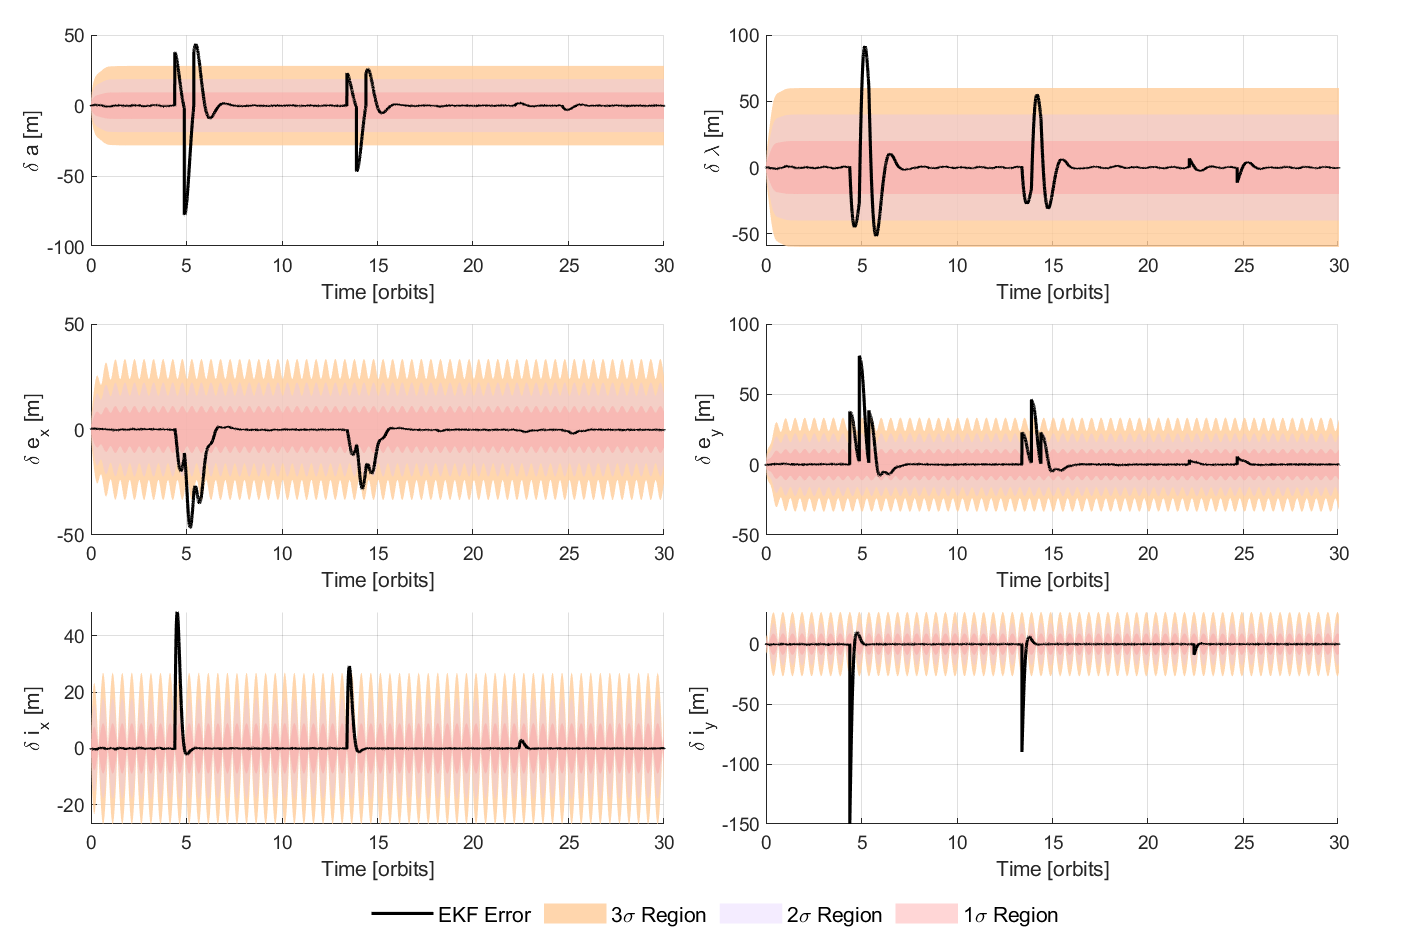
\includegraphics[width=0.7\linewidth]{sim/figures/PS9/EKF_error_SV3.png}
    \caption{SV3 EKF error over time.}
    \label{fig:ekf_error_ps9_sv3}
\end{figure}

Looking at the residuals, we see that a result of the measurement model we get very small residuals in RTN and large residuals in ECI. The measurement step is especially good at reducing the residuals in the RTN position, which is clear in Figure \ref{fig:ekf_residuals_sv3_ps9}.

\begin{figure}[H]
    \centering
    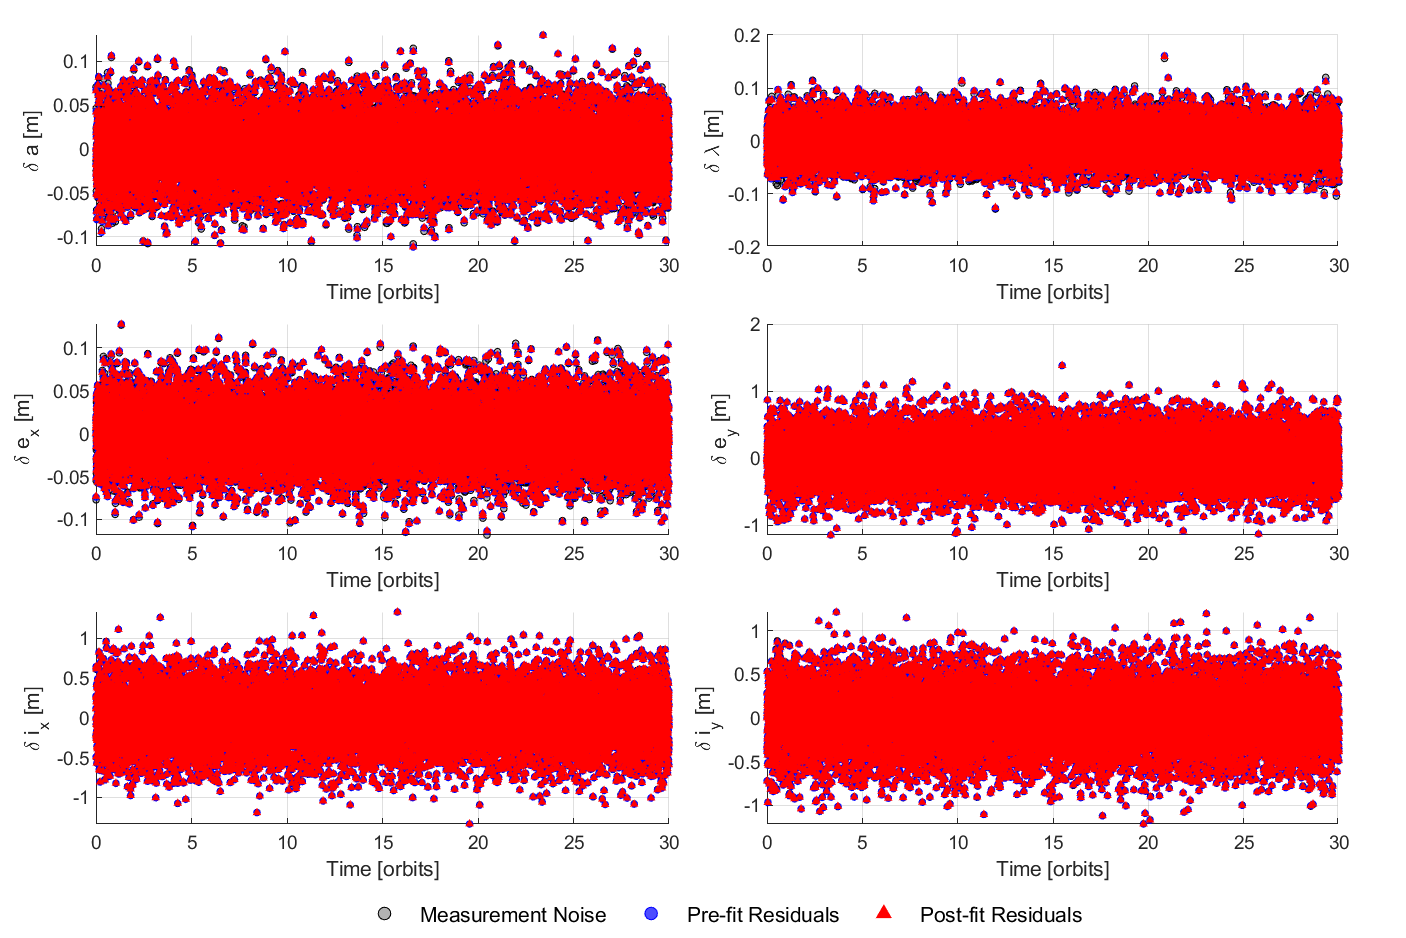
\includegraphics[width=0.7\linewidth]{sim/figures/PS9/residuals_SV2.png}
    \caption{SV2 EKF residuals.}
    \label{fig:ekf_residuals_sv2_ps9}
\end{figure}

\begin{figure}[H]
    \centering
    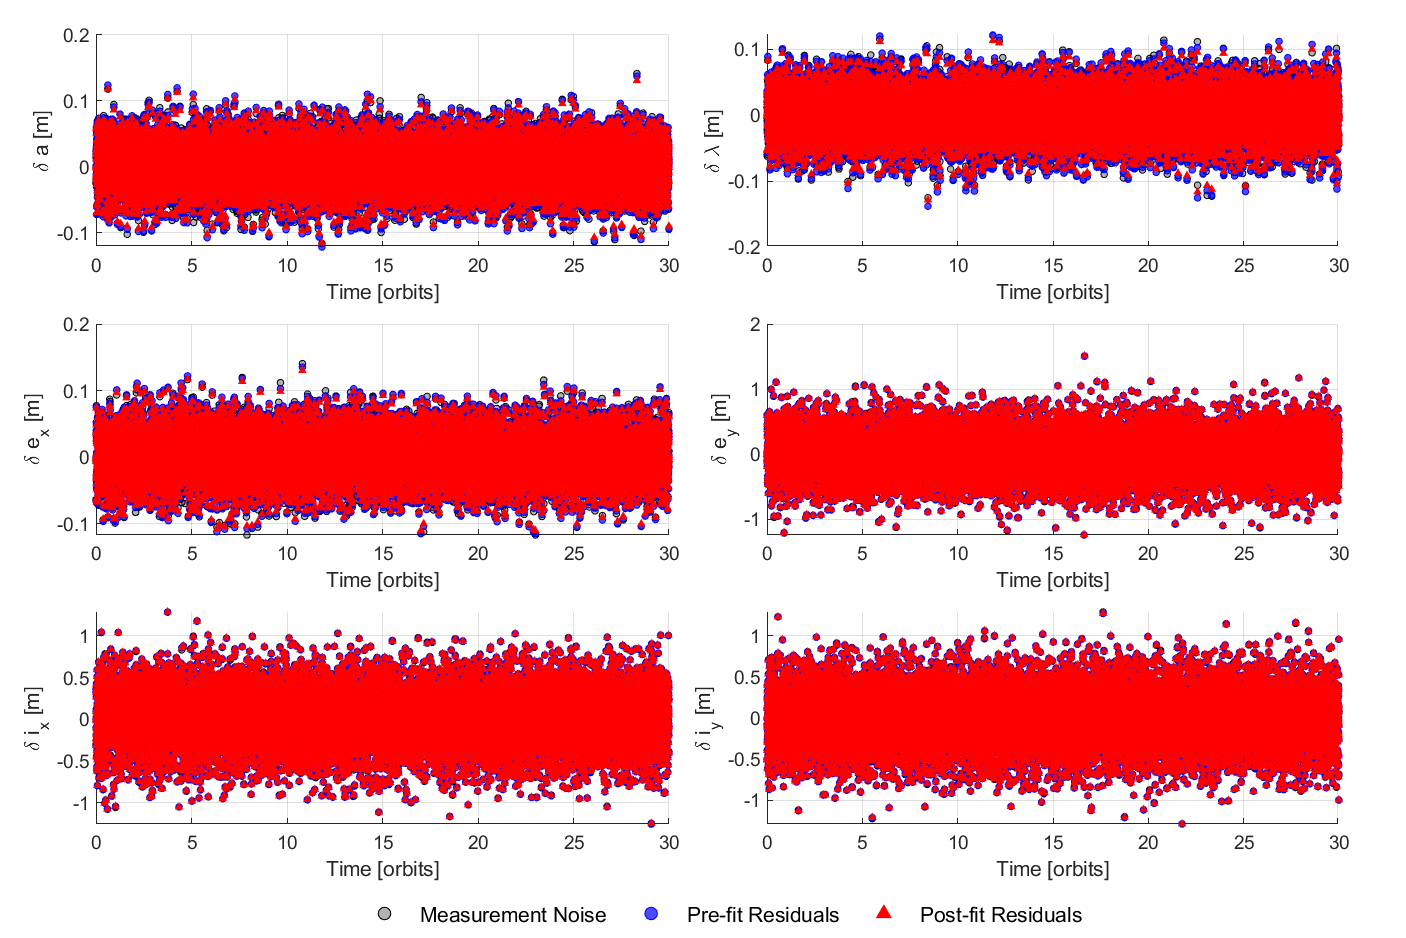
\includegraphics[width=0.7\linewidth]{sim/figures/PS9/residuals_SV3.png}
    \caption{SV3 EKF residuals.}
    \label{fig:ekf_residuals_sv3_ps9}
\end{figure}

Finally, for visualization purposes, we look at the 3D plot of SV1, SV2, and SV3 throughout the simulation, shown in Figure \ref{fig:3d_visual_RTN_final_control}. Despite some drift in the along-track direction, we maintain passive safety and the Docker spacecraft carefully approaches the target while the Watcher watches.

\begin{figure}[H]
    \centering
    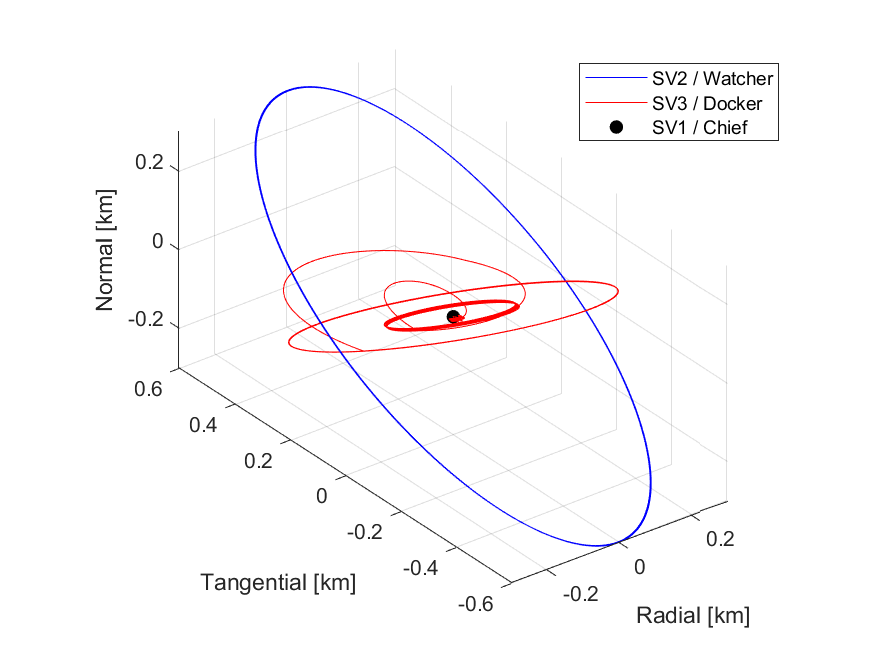
\includegraphics[width=0.7\linewidth]{sim/figures/PS9/ROE_3d_all_maneuvers.png}
    \caption{3D visualization of RTN positions of SV1, SV2, SV3}
    \label{fig:3d_visual_RTN_final_control}
\end{figure}

A useful metric to look at is the error and standard deviation in the final state of SV2 and SV3, given below. As see

\begin{align}
    \mu_{err, SV2}:
\begin{bmatrix} -0.384 \\ 0.607 \\ 0.038 \\ 0.441 \\ -0.171 \\ -0.057 \end{bmatrix} m\\
\mu_{err, SV3}:
\begin{bmatrix} 0.299 \\ 0.637 \\ 0.273 \\ 0.341 \\ 0.139 \\ 0.257 \end{bmatrix} m\\
\sigma_{SV2}:
\begin{bmatrix} -0.142 \\ -0.093 \\ -0.145 \\ 0.045 \\ -0.053 \\ -0.238 \end{bmatrix} m\\
\sigma_{SV3}:
\begin{bmatrix} 9.373 \\ 19.998 \\ 8.500 \\ 10.751 \\ 4.318 \\ 7.814 \end{bmatrix} m
\end{align}

\subsection{Bonus Material}
\subsubsection{Utilizing Radial Burns for Proximity Operations}
We experimented with various different control methods, as highlighted in PS5. One interesting design choice made was to use a more inefficient method pair of radial burns method for our final Mode 4 maneuver. We implemented this despite a working, more efficient tangential burn method for two reasons:
\begin{itemize}
    \item Since radial burns are $2x$ less effective than tangential burns, we get finer control for each impulse bit the thruster can impart. Thus, it becomes a good choice for proximity operations, where the thrust reaction needed would be very small.
    \item Radial burns affect $\delta e$ and thus the $\delta \lambda$ drift. But, radial burns do not impact $\delta a$ unlike tangential burns, which is helpful for controlling the $\delta \lambda$ drift, since it only depends on $\delta e$ rather than both $\delta e$ and $\delta a$.
    \item In practical scenarios, thrusters of our Docker satellite pluming the target satellite would be a major concern. Radial burns avoid that by thrusting in a perpendicular direction.
\end{itemize}

The result of this can be seen in Figure \ref{fig:delta_v_cumulative_sv3}, which shows the radial $\Delta v$ in mode 4.

\subsubsection{Actuator Modeling}
We went about coming up with an approximate model of our larger thruster used for impulsive control. Specifically, we wanted to create a model between the commanded $\Delta v_{cmd}$ and the resultant output $\Delta v_{out}$. Taking our largest $\Delta v$, we can estimate the approximate thrust output of our impulse thruster.

\begin{align}
    \Delta v &= 0.04 m/s \\
    &\implies a = \Delta v dt = 0.41 m/s^2 \\
    &\implies F = ma = 5.5 N
\end{align}

We see that we require around a 5N thruster. Based on \cite{polk2013recommended}, we can say that we would approximately see white noise in the actuator with a standard deviation around $5 mN$ of thrust, $\approx~0.1\%$ of the true value.

In our modeling, we do this by applying a uniform noise between $\pm k_{noise} \%$ to the commanded thrust value for the impulse burns. While experimenting with different values of $k_{noise}$, we noticed that $0.1\%$ has a negligible effect on our results. For lack of repetition, those plots are excluded. However, to see an extreme case, we explored adding $10\%$ noise to the impulse burns. The 3D visualization for this is shown in Figure \ref{fig:3d_vis_with_act_noise}.

\begin{figure}[H]
    \centering
    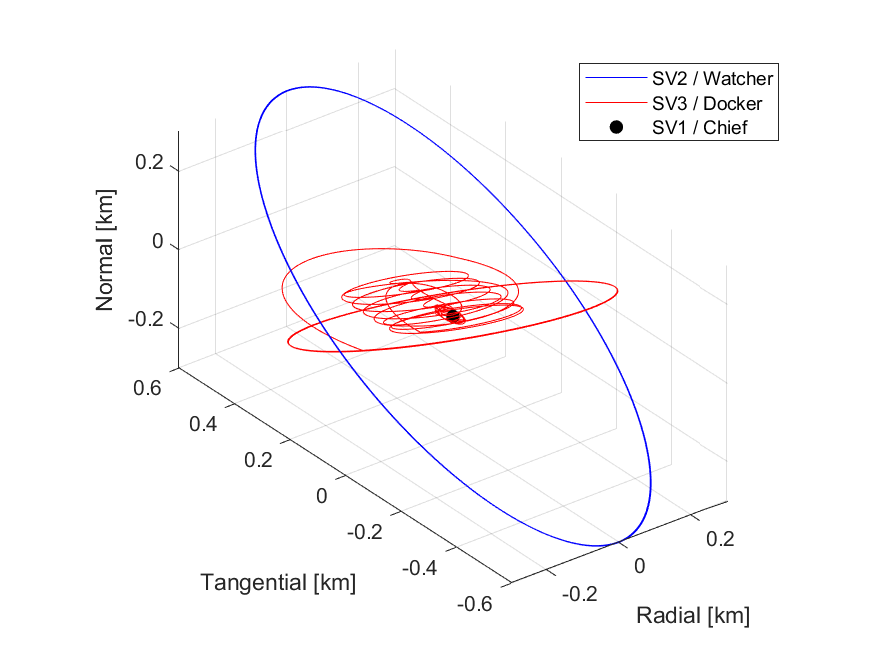
\includegraphics[width=0.75\linewidth]{sim/figures/PS9/ROE_3d_all_maneuvers_act_noise.png}
    \caption{3D visualization of RTN positions of SV1, SV2, SV3, with 10\% noise added to impulsive burns.}
    \label{fig:3d_vis_with_act_noise}
\end{figure}

We can see that this change to the thrust results in poor maneuvers, which in turn lead to more of a drift in the relative mean longitude that has to be corrected by the continuous control during station keeping. As a result, the $\Delta v$ increased slightly. Although the difference is noticeable, we were surprised that the effect was not more drastic for smaller noise levels.
In reality, such a thruster would also have some delay in thrust output, second order effects in its valve response, etc. However, since our time-step for the simulation is very large relative to the time for thruster actuation, these effects would not be possible to simulate.

\subsubsection{Dynamic Q Tuning}
As shown in Figure \ref{fig:ekf_error_ps9_sv3}, there is a spike in the estimate error of the relative orbital elements during and around the large impulsive maneuvers for SV3. The EKF is too slow to adapt to the larger jumps in the state. Therefore, to get a good estimate even during these impulsive burns, we attempted to increase the process noise significantly, thus making the filter more reliant on the measurements during that phase. The two choices for $Q$ were ($R$ was not changed between the two cases)
\begin{align}
    Q_{base} &= I_{6\times 6} \\
    Q_{high} &= 100I_{6\times 6}
\end{align}
In comparison, the $Q$ value for SV2 is $Q_{SV2} = 10^{-3}I_{6\times 6}$, which allows for smooth estimates that work well because of the lack of large spikes in state.

However, our preliminary experiment with this didn't yield any noticeable changes. Since the modification to $Q$ was only done at a single time-step, its effect was negligible. A more advanced version of this might be to apply the modified $Q$ not just at the single time-step of the impulse, but to apply it around the predicted burns. However, the definition of that is ambiguous and would require some design iterations.

\newpage
\subsection{Conclusion and Way Forward}
\subsubsection{Summary of the Project}
The Servicing and Observing Satellite Swarm (SOSS) aims to demonstrate on-orbit servicing of an uncontrollable target spacecraft with a swarm of one docking satellite and one observing satellite. SOSS is made up of two spacecraft: one Docker spacecraft, which is referred to as SV3, and one Watcher spacecraft, which is referred to as SV2. These two spacecraft work together to service a Target spacecraft, which is referred to as SV1. Overall, the Docker spacecraft approaches, docks, and services the Target spacecraft, while the Watcher spacecraft aids in the Target pose estimation and provides additional safety checks from a constant relative orbit. SOSS is inspired by the NASA Starling swarm which demonstrated the viability of autonomous angles-only vision-based navigation in orbit. As such, SOSS inherited some parameters from Starling, including the absolute orbital elements of the Target spacecraft - as shown in Table \ref{tab:abs_oe_kepler_summary} - and the physical size of the spacecraft in the swarm. 

\begin{table}[h]
\centering
\begin{tabular}{cccccc} \hline
    $a$ & $e$ & $i$ & $\omega$ & $\Omega$ & $\nu$ \\ \hline 
     6944 km & 0.0016 & 99.4 $^\circ$ & 91.432$^\circ$ & -151.1$^\circ$ & -139.45$^\circ$ \\ \hline
\end{tabular}
\caption{Initial Keplerian Orbit Parameters of the Target spacecraft}
\label{tab:abs_oe_kepler_summary}
\end{table}

The Target spacecraft is chosen as the chief spacecraft with the Docker and Watcher spacecraft acting as two deputy spacecraft since their motion relative to the Target spacecraft is most important in the rendezvous, proximity, and docking operations. The Target spacecraft (SV1) has no maneuvering capabilities as it has run out of propellant, and our formation is aiming to refuel it. As such, SV1 will act as the origin of the relative Radial-Tangential-Normal (RTN) frame and remain there throughout all of our operational modes. The Watcher spacecraft (SV2) has sensing capabilities, including optical cameras such as those in the NASA Starling mission, which will be used to inspect the Target and estimate its pose for servicing purposes. The Docker spacecraft (SV3) also has optical sensors that will aid in this inspection, but also play a crucial role in proximity and docking operations. Our formation aims to demonstrate a significant advance in on-orbit pose estimation and characterization of objects, along with improved docking operations through the use of multiple spacecraft with a variety of sensor modalities. Further details can be found in Problem Set 1. 

Throughout the project, quasi-nonsingular Relative Orbital Elements (ROEs) are used to characterize relative motion. ROEs are defined by D'Amico as a function of the orbit elements of the target $t$ and observer $o$ spacecraft.\cite{damicothesis} They are given by:
\begin{align}
\delta \boldsymbol{\alpha} &= 
\begin{bmatrix} \label{eq:quasi_nonsign_roe}
\delta a & \delta \lambda & \delta e_x & \delta e_y & \delta i_x & \delta i_y
\end{bmatrix}^\top \notag \\
&= 
\left( 
\begin{bmatrix}
\delta a \\
\delta \lambda \\
|\delta\mathbf{e}| \cos \phi \\
|\delta\mathbf{e}| \sin \phi \\
|\delta\mathbf{i}| \cos \theta \\
|\delta\mathbf{i}| \sin \theta
\end{bmatrix}
= 
\begin{bmatrix}
\frac{a_t - a_o}{a_o} \\
(u_t - u_o) + (\Omega_t - \Omega_o) \cos i_o \\
e_{x,t} - e_{x,o} \\
e_{y,t} - e_{y,o} \\
i_t - i_o \\
(\Omega_t - \Omega_o) \sin i_o
\end{bmatrix}
\right)
\end{align}

where $[\delta e_x, \delta e_y]$ are components of the relative eccentricity vector with phase $\phi$ and $[\delta i_x, \delta i_y]$ are components of the relative inclination vector with phase $\theta$.

The first part of the project investigated the various dynamic models that can be used to propagate absolute and relative orbits with and without J2 perturbations. First, the Fundamental Orbital Differential Equation (FODE) was used to propagate the absolute orbit of the chief spacecraft with and without J2 perturbations using a custom Runge-Kutta integrator with a fixed time step of approximately 11 seconds or $\frac{1}{500}$ of the orbit period to ensure accuracy. Figure \ref{fig:3d_plots_with_j2} shows the 3D plot of the orbit in an inertial frame, and compares the orbit with and without J2 perturbations, but propagated for 200 orbits to illustrate the change in the argument of periapsis. 

\begin{figure}[H]
    \centering
    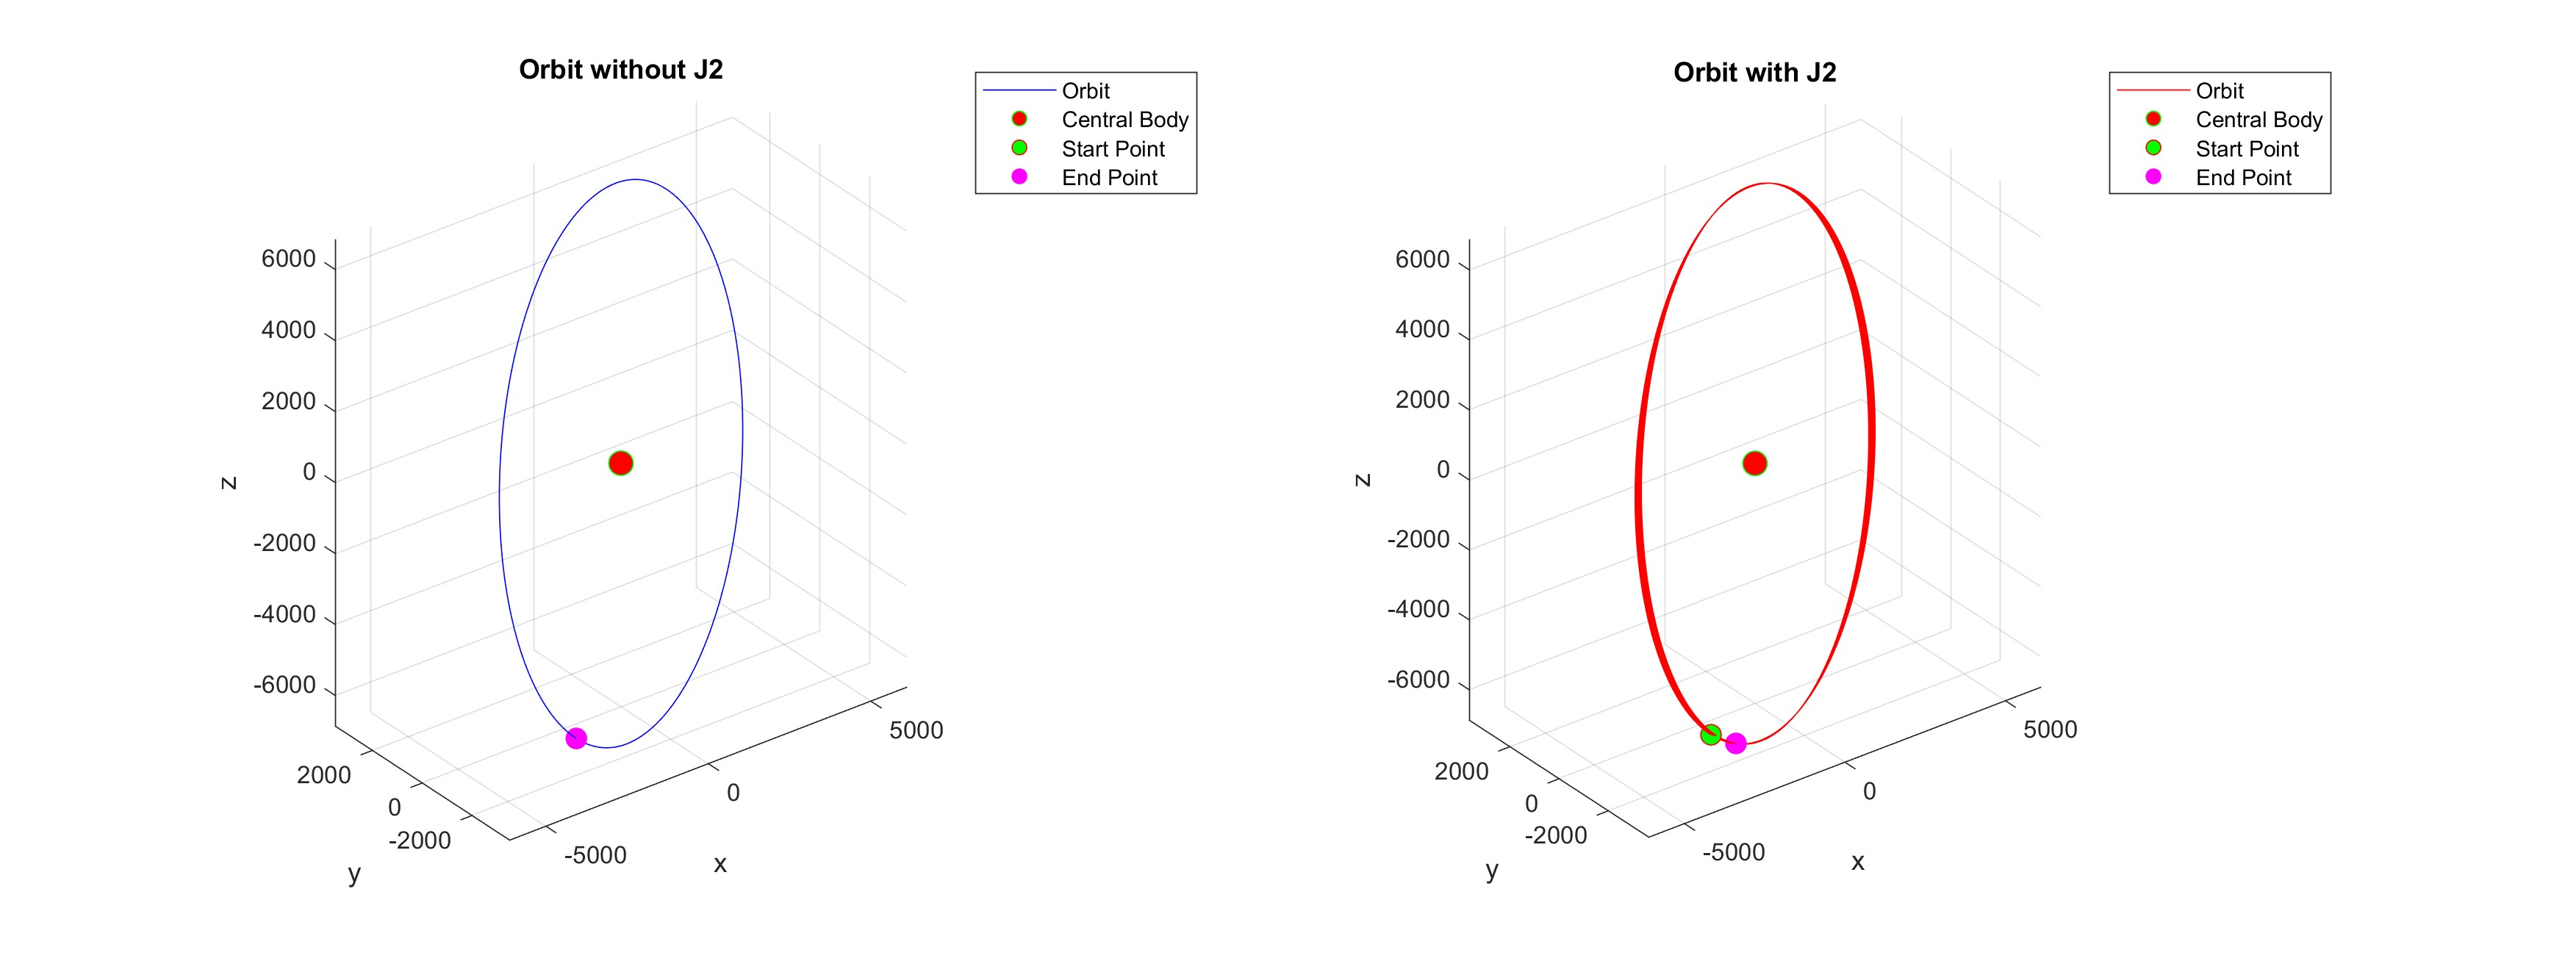
\includegraphics[width=1.1\linewidth]{PS1/Figures/Orbit_J2_Comparison_ECI.jpg}
    \caption{Comparison of the 3D plots with (right) and without (left) J2 perturbations. }
    \label{fig:3d_plots_with_j2}
\end{figure}

These results from FODE were compared to an analytical Keplerian propagator, which showed that numerical errors begin to accumulate as the simulation time goes on. Next, the osculating and mean orbital elements with J2 effects were analyzed and as expected they tracked with each other. The mean orbital elements reflect only the secular effects of J2, while the osculating elements include periodic effects. More details can be found in Problem Set 1.

Then, in Problem Set 2, the relative orbit derived from non-linear integration of the Fundamental Equation of Relative Motion (FERM) was compared to the one derived from FODE. As expected, both methods produce the same results with negligible numerical errors, even with different initial conditions, such as a non-zero relative semi-major axis difference. Additionally, an impulsive maneuver to correct for the relative semi-major axis difference was derived and successfully applied. This is important because bounded periodic relative motion between a deputy and chief spacecraft arises from the specific mechanical energies of their orbits being equal - a condition known as "energy matching" - and this only occurs when the semi-major axes of the chief and deputy orbits are the same. In other words, when the semi-major axes are different, each spacecraft has a different mean motion about its orbit, which leads to them gradually drifting away from each other in the relative frame, specifically in the tangential direction. Further details can be found in Problem Set 2. 

In Problem Set 3, the Hill-Clohessy-Wiltshire (HCW) and Yamanaka-Ankersen (YA) solutions were explored for near-circular and eccentric orbits, respectively. Also, the geometric linear mapping approach, which maps ROEs from one initial state to a state in the future, was used as a basis of comparison. It was found that the geometric linear mapping apporach was the most accurate. More details can be found in Problem Set 3.

In Problem Set 4, J2 effects were investigated through osculating and mean elements in the RTN and ROE frames. As expected, a non-zero semi-major axis difference leads to drifts in the tangential direction in the RTN frame and in relative eccentricity, relative inclination vectors, and the relative mean longitude in the ROEs. Figure \ref{fig:RTN_projections_summary} shows the relative position projected into the RTN planes with and without J2 effects.

\begin{figure}[H]
    \centering
    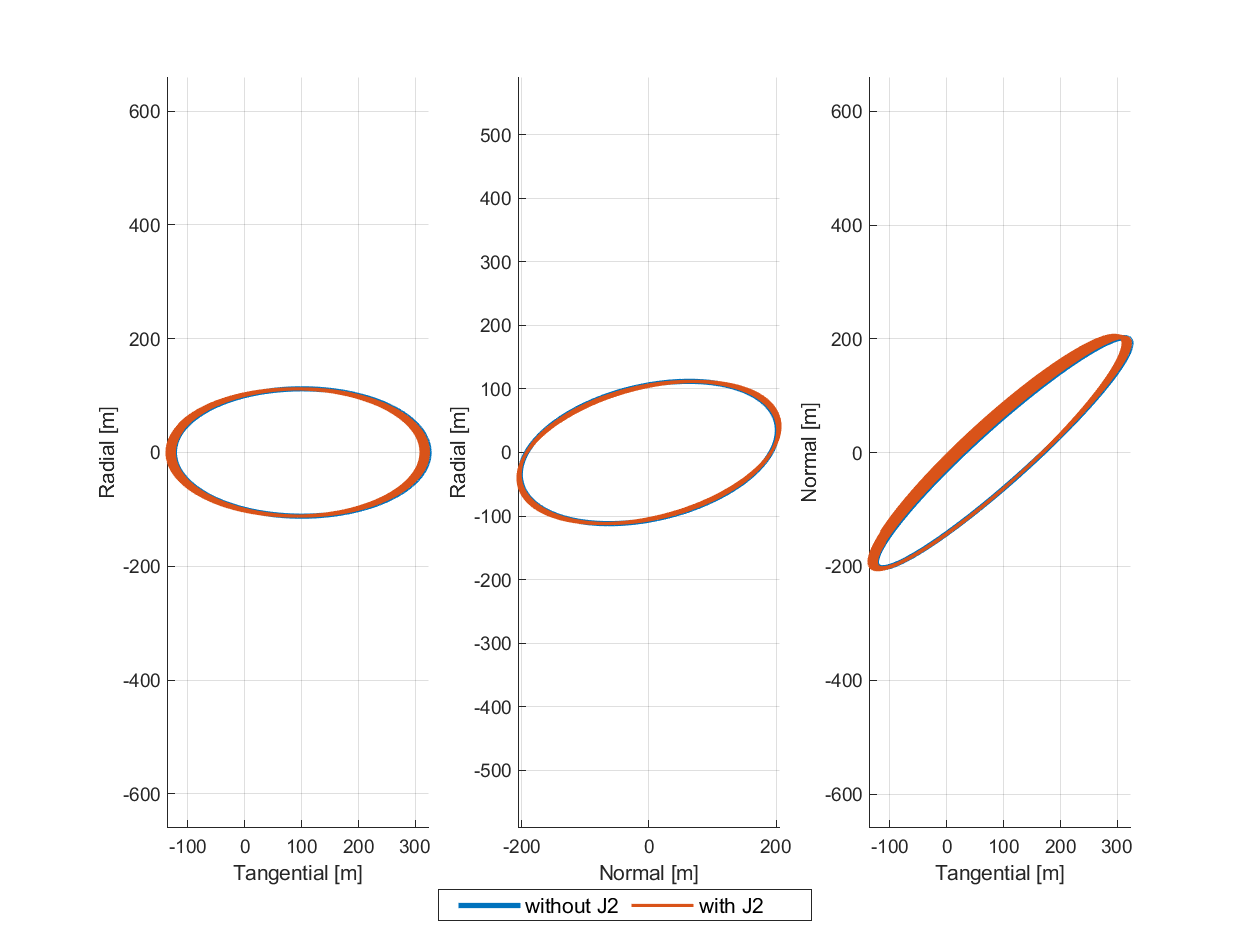
\includegraphics[width=0.75\linewidth]{sim/figures/PS4/RTN_projections_SV2.png}
    \caption{Relative position in RTN projections}
    \label{fig:RTN_projections_summary}
\end{figure}

To understand whether the results are according to our expectations, we need to understand how the relative orbit geometry relates to relative orbital elements. Figure \ref{fig:rel_geometry_summary} shows a figure from the lecture slides. From this, we can see that $\delta a$ determines the center of the relative motion ellipse in the radial direction. $\delta \lambda$ determines the center of the relative motion ellipse in the tangential direction. $\delta e$, which is the L2 norm of $\delta e_x$ and $\delta e_y$, determines the size of this ellipse in the tangential and radial directions. $\delta i$, which is the L2 norm of $\delta i_x$ and $\delta i_y$, determines the size of the ellipse in the normal direction. 

\begin{figure}[H]
    \centering
    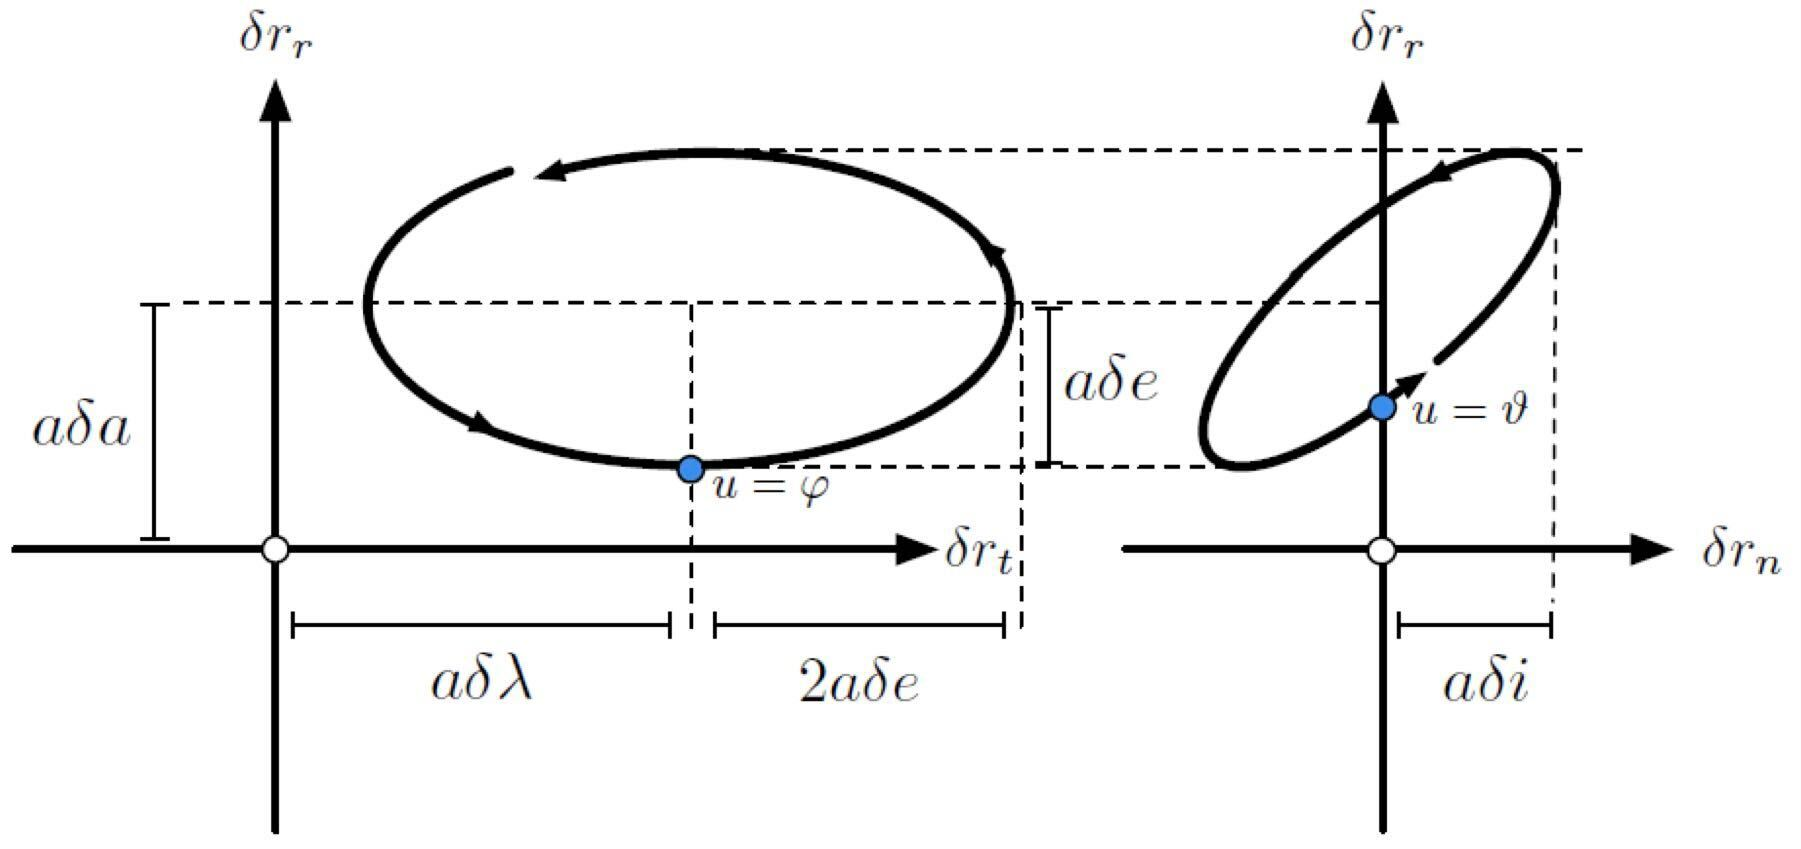
\includegraphics[width=0.75\linewidth]{LaTeX/Figures/RelOrbitGeometry.jpg}
    \caption{Relative orbit geometry}
    \label{fig:rel_geometry_summary}
\end{figure}

Now with that understanding, we look at the effects of J2 on the relative orbital elements. In the quasi-nonsingular relative orbital elements, there are drifts seen in the eccentricity vector $\delta e$, the inclination vector $\delta i$ (specifically the y-component $\delta i_y$), and the mean longitude $\delta \lambda$. The differential J2 effects for near-circular orbits are given by:
\begin{align}
    \frac{d \varphi}{d u} &= \frac{3}{2} \gamma (5\cos^2(i_c) - 1) \\
    \frac{d \delta i_y}{d u} &= 3\gamma \sin^2(i_c) \delta i_x \label{eq:drift_in_rel_i} \\
    \frac{d \delta \lambda}{d u} &= -\frac{21}{2}\left(\gamma \sin(2i_c)\delta i_x 
+ \frac{1}{7} \delta a\right) \label{eq:drift_in_lambda_rel}\\
    \text{where} \quad \gamma  &= \frac{J_2 R_E^2}{2 a^2 (1 - e)^2}
\end{align}
Here, the $\varphi$ is the angle of the eccentricity vector $\delta e$, i.e. $\varphi = \tan^{-1}\left(\frac{\delta e_y}{\delta e_x}\right)$.

Thus, based on these equations and our initial ROE ($\delta a = 0$, $\delta i_x \neq 0$), we expect drifts $\delta i$ and $\delta \lambda$, but not in the magnitude $\delta e$, since only the phase of the relative eccentricity vector is changing, not the magnitude. $\delta i$ has a drift, because J2 only effects the $\delta i_y$ component of the relative inclination vector. From the drift in $\delta \lambda$, we expect to see a drift of the ellipse in the tangential direction in the RTN frame, which is observed. From the drift in the phase of $\delta e$, we expect to see the ellipse starting to rotate as its "relative perigee" drifts circularly. This too is observed in the RTN frame. Thus, the results in the RTN frame are as expected given the initial relative orbital elements. Finally, from the drift in $\delta i$ we expect to see a drift of the ellipse in the normal direction in the RTN frame, which, while not very significant, is also observed. 

Additionally, in Problem Set 4, an analytical solution for J2 effects on ROEs was used to derive a State Transition Matrix (STM), which yielded results that aligned with the non-linear propagation. This informed future decisions on propagation methods to use in the control and navigation algorithms. Further details can be found in Problem Set 4. 

In Problem Set 5, the operational modes, control requirements, choice of actuators, dynamics models, and the impulsive control law via the naive least-squares method were defined, tested, and verified. Note that all of these were subject to change as they were improved upon in our final implementation. As such, only the final operational modes will be discussed here, with the rest discussed in our final navigation and control implementation later in the summary. The significant operational modes of SOSS are as follows: 
\begin{enumerate}
\item \textbf{Initial Checkout Mode} - Initial checkout of Target spacecraft with both Watcher and Docker less than a kilometer and more than 200 meters away at closest approach to allow for vision-based sensing
\item \textbf{Approach Mode} - Docker approaches the Target while Watcher watches from the same distance. This mode runs until the Docker is approximately 10 meters away from the Target
\item \textbf{Proximity Operations Mode} - Docker completes final approach Target while Watcher watches
\item \textbf{Docked Mode} - Docker docks and services Target while Watcher watches
\item \textbf{Station Keeping Mode} - Watcher and Target stay within prescribed limits of relative eccentricity and relative inclination to remain passively safe. This mode will be applied whenever the formation is not reconfiguring. 
\end{enumerate}

These operational modes and minimum separation requirements are translated into ROEs as shown in \ref{tab:roe_modes_summary}. In the swarm design, $\delta e$ and $\delta i$ were chosen to be equal in magnitude for both SV2 and SV3 in order to give circular relative motion, which is helpful for maintaining the same distance throughout an orbit for the vision-based sensing on both spacecraft. Additionally, $\delta e$ and $\delta i$ were chosen to be antiparallel for SV3 (Docker) and parallel for SV2 (Watcher) to ensure that the Docker never blocks the Watcher's view of the Target by tilting the Docker's relative orbit perpendicular to the Watcher's.

Table \ref{tab:roe_modes_summary} outlines the ROEs for each operational mode for each operational mode.
\begin{table}[h!]
\centering
\begin{tabular}{|c|rrrrrr|rrrrrr|}
\hline
\textbf{Mode} & \multicolumn{6}{c|}{\textbf{Watcher (SV2) [m]}} & \multicolumn{6}{c|}{\textbf{Docker (SV3) [m]}} \\
\cline{2-13}
 & $d_a$ & $d_\lambda$ & $d_{e_x}$ & $d_{e_y}$ & $d_{i_x}$ & $d_{i_y}$ 
 & $d_a$ & $d_\lambda$ & $d_{e_x}$ & $d_{e_y}$ & $d_{i_x}$ & $d_{i_y}$ \\
\hline
1 & 0 & 0 & 0 & 300 & 0 & 300 & 0 & 0 & 0 & 250 & 0 & -250 \\
2 & 0 & 0 & 0 & 300 & 0 & 300 & 0 & 0 & 0 & 100 & 0 & -100 \\
3 & 0 & 0 & 0 & 300 & 0 & 300 & 0 & 0 & 0 & 10  & 0 & -10 \\
4 & 0 & 0 & 0 & 300 & 0 & 300 & 0 & 0 & 0 & 1   & 0 & -1 \\
\hline
\end{tabular}
\caption{Relative Orbital Element Modes for SV2 and SV3 (scaled by $a_c$)}
\label{tab:roe_modes_summary}
\end{table}

Implementing the ground-truth model in open-loop shows each desired mode in the RTN planes as shown in Figures \ref{fig:mode_1_rtn}, \ref{fig:mode_2_rtn}, \ref{fig:mode_3_rtn}. Note that Mode 4 is not shown because SV3 does not appear in the plots due to its ROE all being 0. This ground-truth model exhibits expected J2 perturbations with a drifting relative perigee. Also note how the inclinations of the relative orbits are offset in the NT projection due to the design choice of antiparallel relative eccentricity and relative inclination vectors of SV3. All of these modes exhibit passive safety through $e$-$i$ vector separation. Passive safety ensures that if control of a spacecraft is lost and it drifts tangentially, it will not collide with the other spacecraft. This is achieved specifically through the relative eccentricity and relative inclination vectors being aligned in parallel or antiparallel directions. 

% --- Mode 1 ---
\begin{figure}[H]
    \centering
    \begin{subfigure}[b]{0.32\linewidth}
        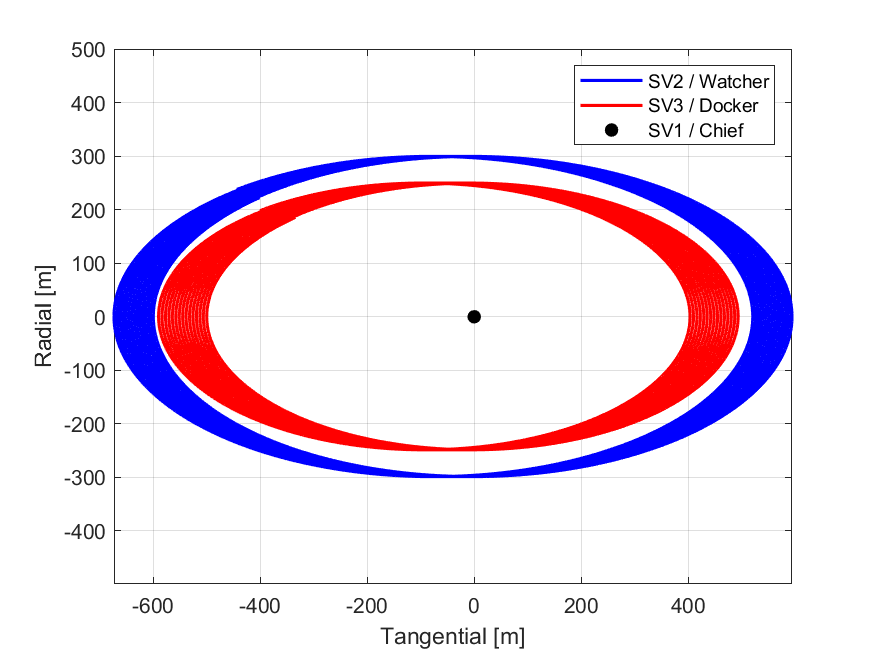
\includegraphics[width=\linewidth]{sim/figures/PS5/mode_1_RTN.png_RT.png}
        \caption{RT Projection}
        \label{fig:mode_1_rt}
    \end{subfigure}
    \begin{subfigure}[b]{0.32\linewidth}
        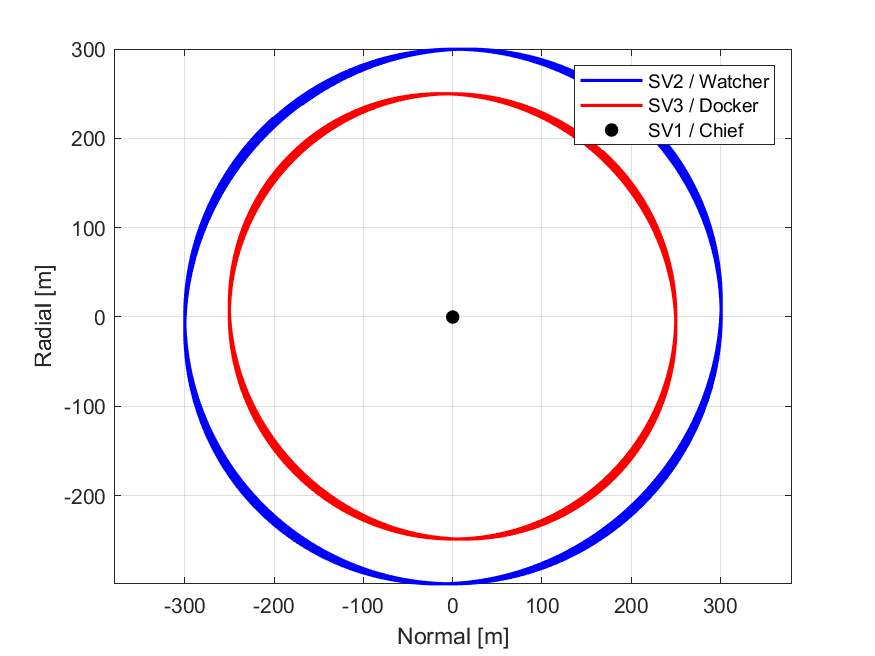
\includegraphics[width=\linewidth]{sim/figures/PS5/mode_1_RTN.png_RN.png}
        \caption{RN Projection}
        \label{fig:mode_1_rn}
    \end{subfigure}
    \begin{subfigure}[b]{0.32\linewidth}
        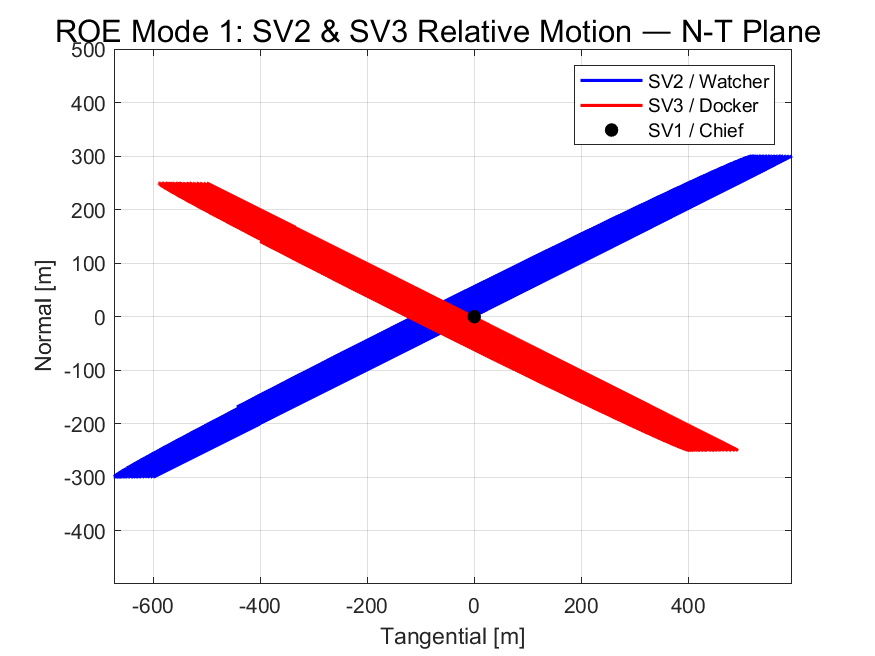
\includegraphics[width=\linewidth]{sim/figures/PS5/mode_1_RTN.png_NT.png}
        \caption{NT Projection}
        \label{fig:mode_1_nt}
    \end{subfigure}
    \caption{Mode 1 RTN Projections}
    \label{fig:mode_1_rtn}
\end{figure}

% --- Mode 2 ---
\begin{figure}[H]
    \centering
    \begin{subfigure}[b]{0.32\linewidth}
        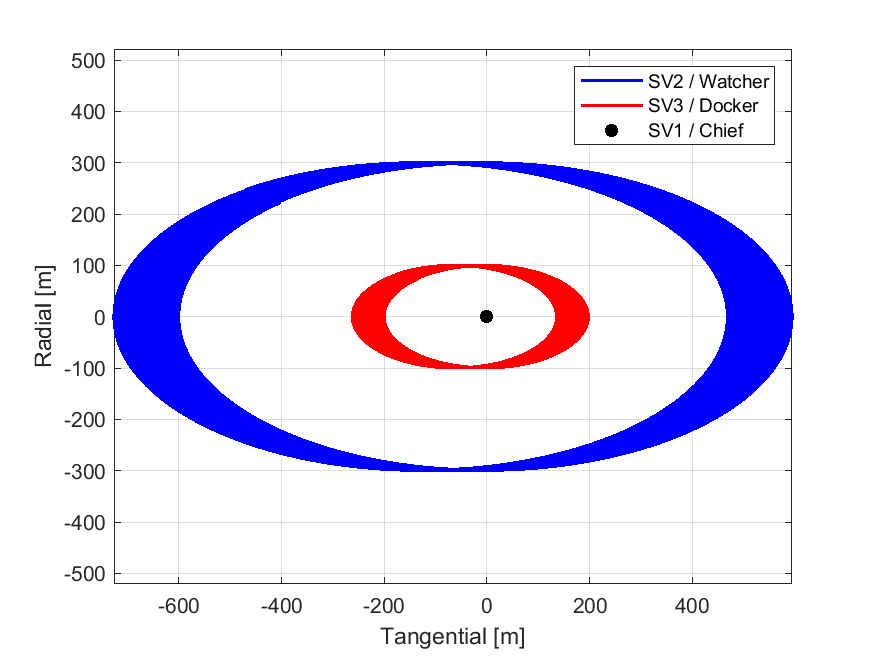
\includegraphics[width=\linewidth]{sim/figures/PS5/mode_2_RTN.png_RT.png}
        \caption{RT Projection}
        \label{fig:mode_2_rt}
    \end{subfigure}
    \begin{subfigure}[b]{0.32\linewidth}
        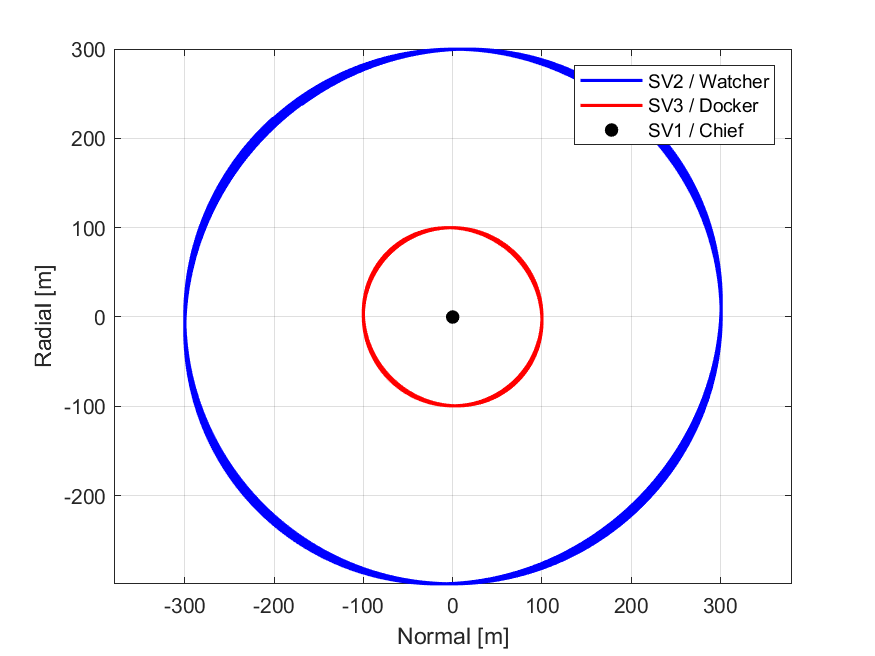
\includegraphics[width=\linewidth]{sim/figures/PS5/mode_2_RTN.png_RN.png}
        \caption{RN Projection}
        \label{fig:mode_2_rn}
    \end{subfigure}
    \begin{subfigure}[b]{0.32\linewidth}
        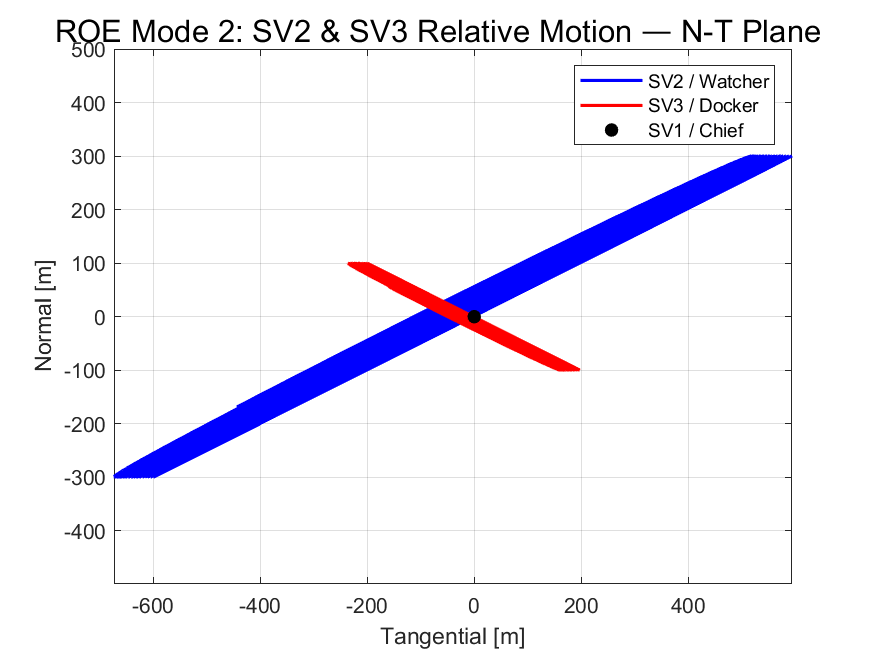
\includegraphics[width=\linewidth]{sim/figures/PS5/mode_2_RTN.png_NT.png}
        \caption{NT Projection}
        \label{fig:mode_2_nt}
    \end{subfigure}
    \caption{Mode 2 RTN Projections}
    \label{fig:mode_2_rtn}
\end{figure}

% --- Mode 3 ---
\begin{figure}[H]
    \centering
    \begin{subfigure}[b]{0.32\linewidth}
        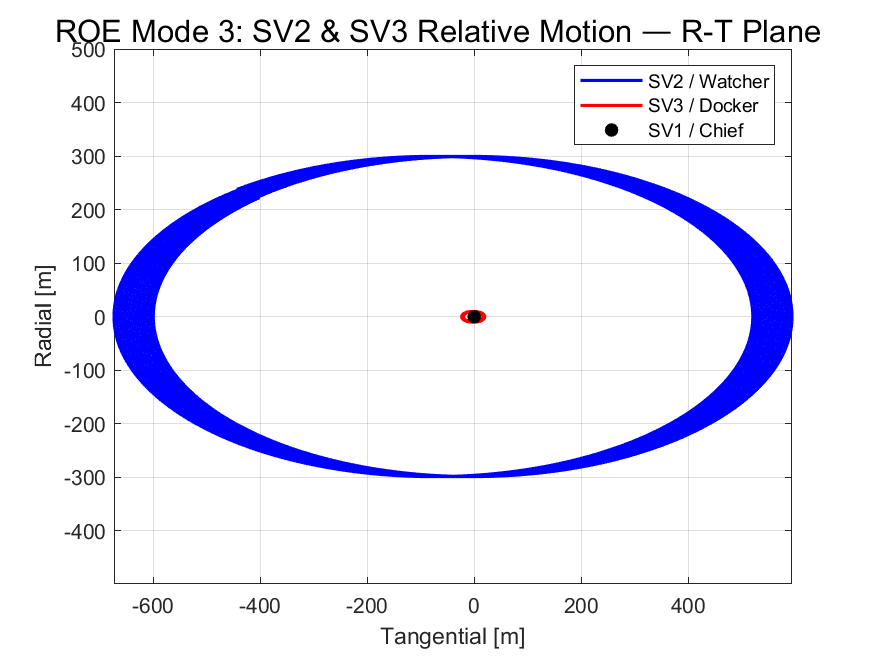
\includegraphics[width=\linewidth]{sim/figures/PS5/mode_3_RTN.png_RT.png}
        \caption{RT Projection}
        \label{fig:mode_3_rt}
    \end{subfigure}
    \begin{subfigure}[b]{0.32\linewidth}
        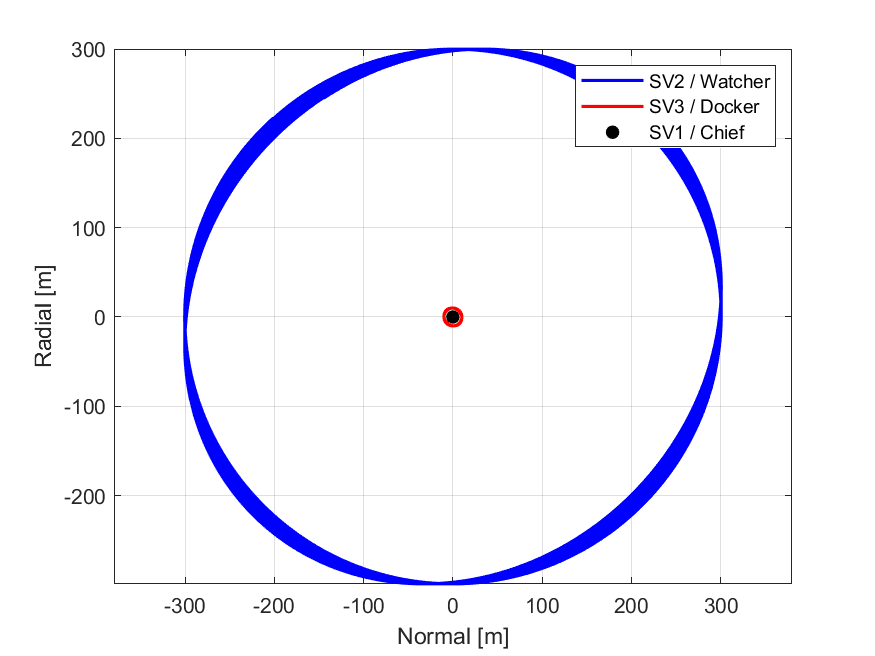
\includegraphics[width=\linewidth]{sim/figures/PS5/mode_3_RTN.png_RN.png}
        \caption{RN Projection}
        \label{fig:mode_3_rn}
    \end{subfigure}
    \begin{subfigure}[b]{0.32\linewidth}
        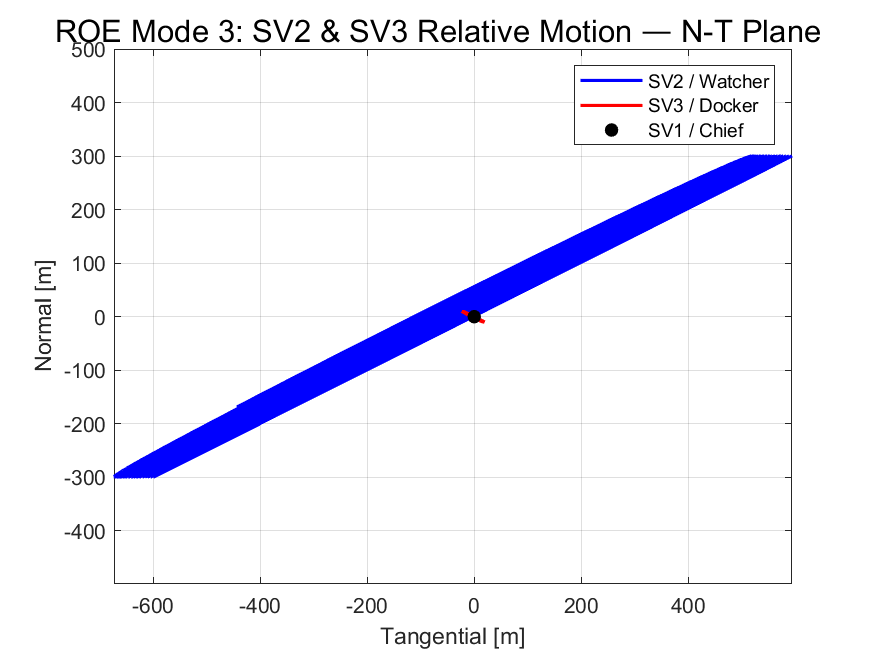
\includegraphics[width=\linewidth]{sim/figures/PS5/mode_3_RTN.png_NT.png}
        \caption{NT Projection}
        \label{fig:mode_3_nt}
    \end{subfigure}
    \caption{Mode 3 RTN Projections}
    \label{fig:mode_3_rtn}
\end{figure}

In Problem Set 6, continuous control using the Lyapunov control formulation was implemented and successfully tested. Similar to Problem Set 5, the final implementation of navigation and control improved upon the material in Problem Set 6, so it will be discussed further later on in the summary.

In Problem Sets 7 and 8, the navigation system was designed, implemented, and tested without being integrated with control. An Extended Kalman Filter (EKF) was chosen to account for the nonlinearities inherent in orbital dynamics. An Unscented Kalman Filter (UKF) could also be used, but is much more computationally expensive than an EKF. The EKF was shown to track the ground truth propagation well with injected noise and simulated absolute and relative measurements, all without implementing any control. Further details can be found in Problem Sets 7 and 8.

Finally, in Problem Set 9, we implemented the complete integrated navigation and control architecture. For the ground truth, the absolute orbital elements of the chief and deputy spacecraft are propagated using the Gauss Variational Equations (GVEs) with the force model taking into account J2 and drag effects. 

Maneuvers are planned using the estimates from the EKF with a hybrid impulsive and continuous control architecture. Impulsive maneuvers (semi-analytical closed-form methods) were used for the large orbit reconfigurations. This is where a large, high-thrust low-ISP thruster like a chemical rocket engine could be used. Continuous control (Lyapunov-based control) was used for station keeping and reducing any drift left from the impulse maneuvers. This is where low-thrust high-Isp thrusters, such as Hall-effect thrusters, could be used. Also, continuous control is used for station-keeping due to the minimum impulse bit requirements likely being smaller than what chemical propulsion could provide, since station-keeping maneuvers are very small. The estimates of the deputy states from the EKF were used in planning and control.

Measurements are generated from the ground truth by converting absolute orbital elements into absolute ECI measurements and relative RTN measurements of the deputy spacecraft, and adding representative noise. These measurements simulate measurements that could be obtained from a combination of on-board GPS, crosslink, and celestial object measurements. The measurement vector is given as ECI and RTN measurements for each deputy stacked together with some added noise. 
\begin{align}
    y &= \begin{bmatrix}
        y_{SV2} \\
        y_{SV3}
    \end{bmatrix} \\
    &= \begin{bmatrix}
        \boldsymbol{r_{SV2}}^{RTN}\\
        \boldsymbol{r_{SV2}}^{ECI} \\
        \boldsymbol{r_{SV3}}^{RTN} \\
        \boldsymbol{r_{SV3}}^{ECI} \\
    \end{bmatrix}_{12\times 1} + V_t
\end{align}

From here, the measurement sensitivity matrix can be defined to be used in the EKF.
\begin{align}
    C_t = \left.\begin{bmatrix}
        \mathcal{J}a_1 & 0_{3\times6} \\
         Q^\top_{eci2rtn} \mathcal{J}
a_1 & 0_{3\times6} \\
        0_{3\times6}  & \mathcal{J}a_1 \\
        0_{3\times6} & Q^\top_{eci2rtn} \mathcal{J}
a_1\\
    \end{bmatrix} \right|_{x = \bar{x}_t}
\end{align}
where $\mathcal{J}$ is the matrix that converts ROEs to RTN values. 

The state used in the EKF is made up of the ROEs of both deputies (SV2 and SV3) stacked together.
\begin{equation}
\begin{bmatrix}
\delta \boldsymbol{\alpha}_2 \\
\hline
\delta \boldsymbol{\alpha}_3
\end{bmatrix}
=
\begin{bmatrix}
\delta a_2 \\
\delta \lambda_2 \\
\delta e_{x,2} \\
\delta e_{y,2} \\
\delta i_{x,2} \\
\delta i_{y,2} \\
\hline
\delta a_3 \\
\delta \lambda_3 \\
\delta e_{x,3} \\
\delta e_{y,3} \\
\delta i_{x,3} \\
\delta i_{y,3}
\end{bmatrix}
\end{equation}

The EKF uses an STM to propagate the estimated ROE state forward, which is defined as
\begin{align}
    \boldsymbol{\alpha_{\tau}} = \Phi^{J_2}_{\text{qns}}(\alpha_c(t_i), \tau) \boldsymbol{\alpha_{i}} \label{eq:state_transition_relation}
\end{align}

where $\Phi^{J_2}_{\text{qns}}(\alpha_c(t_i), \tau)$ is the state-transition matrix (STM) at time $\tau$, and $\boldsymbol{\alpha_{i}}$ are the initial conditions of the relative orbital elements.

The state-transition matrix for quasi-nonsingular relative orbital elements is given by
\begin{align}
&\Phi^{J_2}_{\text{qns}}(\alpha_c(t_i), \tau) = \nonumber \\ 
&\begin{bmatrix}
1 & 0 & 0 & 0 & 0 & 0 \\
-\left( \frac{3}{2}n + \frac{7}{2} \kappa E P \right)\tau & 1 & \kappa e_{x_i} F G P \tau & \kappa e_{y_i} F G P \tau & -\kappa F S \tau & 0 \\
\frac{7}{2} \kappa e_{y_f} Q \tau & 0 & \cos(\dot{\omega} \tau) - 4\kappa e_{x_i} e_{y_f} G Q \tau & -\sin(\dot{\omega} \tau) - 4\kappa e_{y_i} e_{y_f} G Q \tau & 5\kappa e_{y_f} S \tau & 0 \\
-\frac{7}{2} \kappa e_{x_f} Q \tau & 0 & \sin(\dot{\omega} \tau) + 4\kappa e_{x_i} e_{x_f} G Q \tau & \cos(\dot{\omega} \tau) + 4\kappa e_{y_i} e_{x_f} G Q \tau & -5\kappa e_{x_f} S \tau & 0 \\
0 & 0 & 0 & 0 & 1 & 0 \\
\frac{7}{2} \kappa S \tau & 0 & -4 \kappa e_{x_i} G S \tau & -4 \kappa e_{y_i} G S \tau & 2 \kappa T \tau & 1
\end{bmatrix} \label{eq:stm_matrix}
\end{align}

where we have the following variables
\begin{align*}
\eta &= \sqrt{1 - e^2} &
\kappa &= \frac{3}{4} \frac{J_2 R_E^2 \sqrt{\mu}}{a^{7/2} \eta^4} &
E &= 1 + \eta \\
F &= 4 + 3\eta &
G &= \frac{1}{\eta^2} & \\
P &= 3\cos^2(i) - 1 &
Q &= 5\cos^2(i) - 1 &
R &= \cos(i) \\
S &= \sin(2i) &
T &= \sin^2(i) &
U &= \sin(i) \\
V &= \tan(i/2) &
W &= \cos^2(i/2)
\end{align*} 

The initial estimated mean and covariance were chosen to introduce a small offset from the ground truth values. Similarly, the process noise $Q$ and measurement noise $R$ were tuned to be positive definite and diagonal matrices that represented confidence in the dynamics prediction and realistic measurement noise. 

Putting this all together, our simulation loop has the following structure:
\begin{itemize}
    \item Propagate the ground truth states for SV1, SV2, and SV3. 
    \item Plan maneuvers. 
    \item Apply the control action. This is applied as a $\Delta v$ to the state. As discussed in the bonus section, some noise was added to the actuator as another source of application uncertainty.
    \item Generate measurements based on the measurement model previously discussed, and the ground truth values from SV1, SV2, SV3.
    \item Use the measurements and prior states to generate an estimate of SV2 and SV3's ROEs using our Extended Kalman Filter implementation. These estimates are then used for planning.
\end{itemize}

The full order of operations was critical to ensure that the correct values for the ground truth and the estimates were used for planning, so as to prevent any control or estimation instabilities due to a time delay. This is shown in detail in Figure \ref{fig:nav_control_arch_summary}.

\begin{figure}[H]
    \centering
    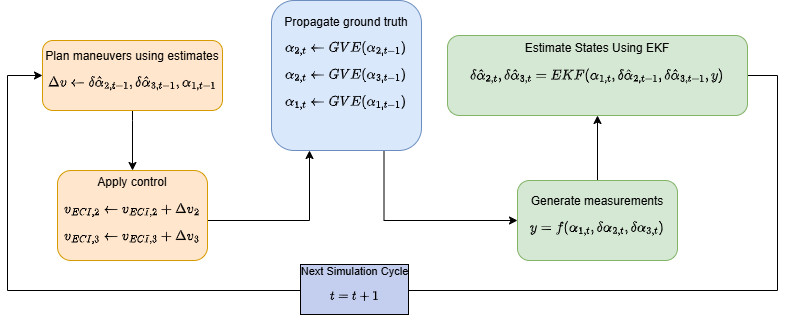
\includegraphics[width=0.85\linewidth]{LaTeX/PS9/soss_control_nav_arch.png}
    \caption{The complete control, simulation, and navigation architecture}
    \label{fig:nav_control_arch_summary}
\end{figure}

The final results will be explored in the next section. More details on the exact formulation of the entire control and navigation architecture can be found in Problem Sets 7, 8, and 9. 

\subsubsection{Assessment of Final Results}


\begin{figure}[H]
    \centering
    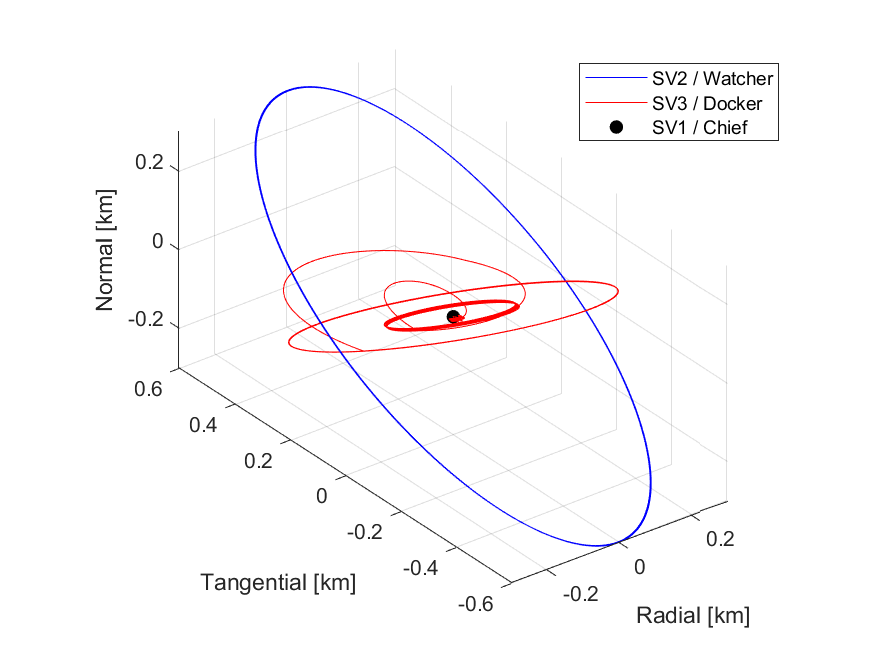
\includegraphics[width=0.75\linewidth]{sim/figures/PS9/ROE_3d_all_maneuvers.png}
    \caption{3D visualization of RTN positions of SV1, SV2, SV3.}
    \label{fig:3d_vis_final_summary}
\end{figure}

\begin{figure}[H]
    \centering
    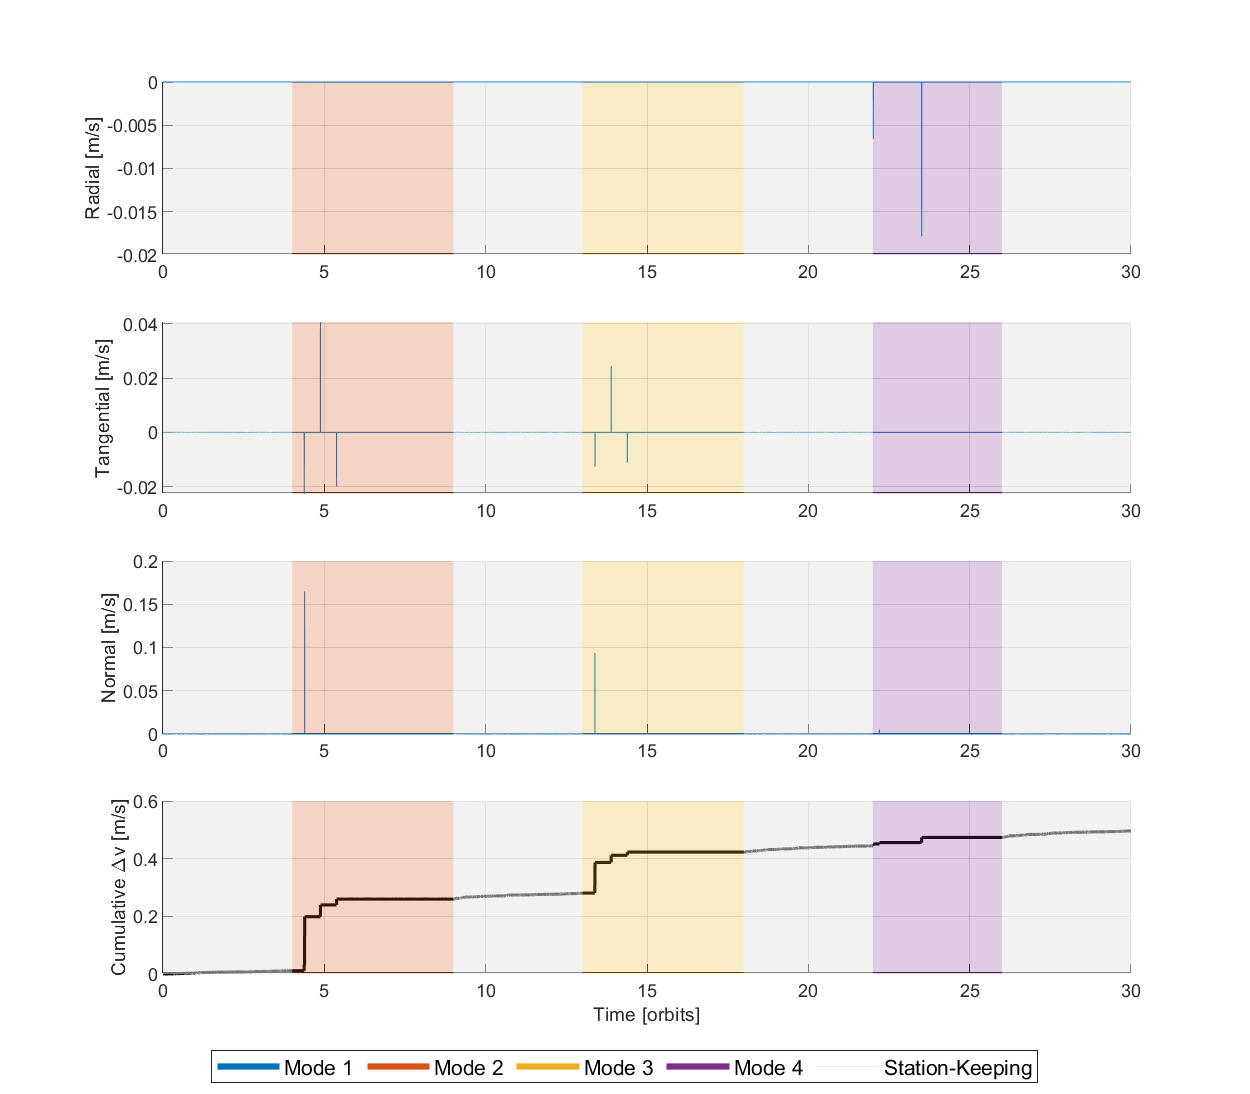
\includegraphics[width=0.7\linewidth]{sim/figures/PS9/delta_v_cumulative_timeline_modes_SV3.png}
    \caption{$\Delta v$ over time for SV3. Note that this uses impulsive control for the maneuvers, but continuous control for station keeping.}
    \label{fig:delta_v_cumulative_sv3_final_sumary}
\end{figure}

\begin{figure}[H]
    \centering
    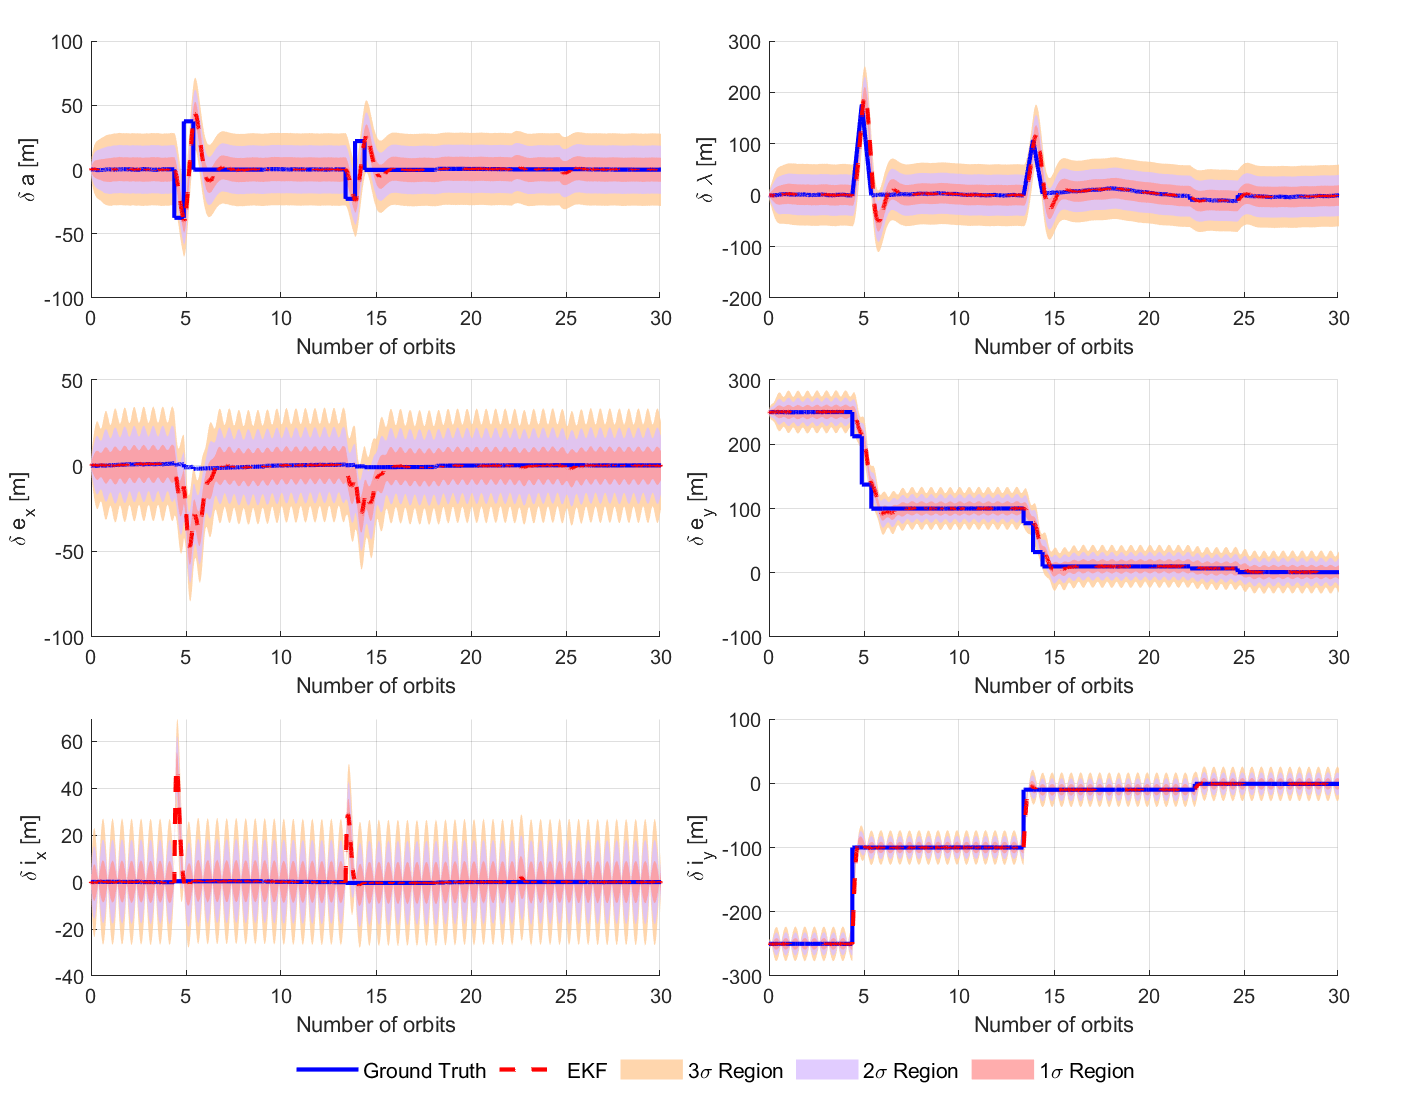
\includegraphics[width=0.7\linewidth]{sim/figures/PS9/ROE_over_time_SV3_comparison.png}
    \caption{True ROEs, estimate ROEs, and covariance bounds for SV3 over time.}
    \label{fig:sv3_ekf_comparison_ps9_final_summary}
\end{figure}

\begin{figure}[H]
    \centering
    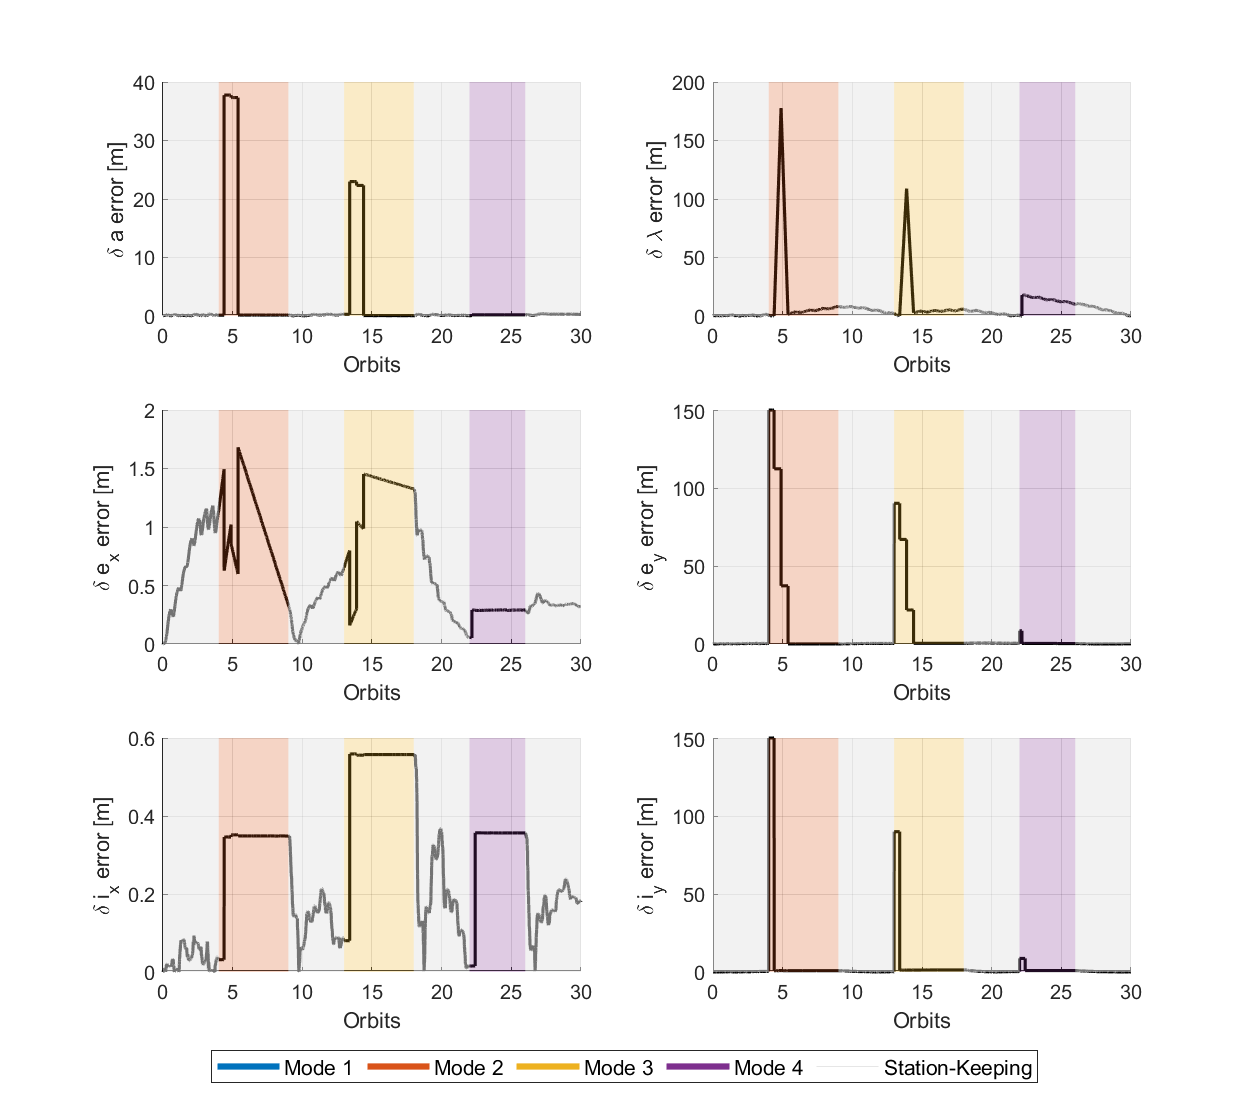
\includegraphics[width=0.7\linewidth]{sim/figures/PS9/ROE_error_over_time_modes_SV3.png}
    \caption{Error between the true ROEs and the desired ROEs for SV3}
    \label{fig:roe_error_control_sv3_summary}
\end{figure}

\subsubsection{Lessons Learned}
Over the course of this project, we have learned an immense amount about the dynamics, navigation, and control of distributed space systems. Some of the key concepts include ROEs and their geometry, the RTN frame, differences between dynamics models and their propagation methods (i.e. FODE vs. FERM vs. GVE vs. STM), the effects of J2 and other perturbations in the ROE and RTN frames, passive safety through $e$-$i$ vector separation, closed-form impulsive and continuous control schemes, the implementation of an EKF with control integration, convex optimization, reachable set theory, angles-only navigation, applications to real-world space missions, and many more. Along with awareness of all the intricate equations and methodologies that power distributed space systems, we have developed an intuitive understanding of relative orbital dynamics, navigation, and control. This intuition will be key to our future careers in engineering.

We also learned a lot of specific lessons concerning best practices for implementation. First, the conversions between degrees and radians must be marked and kept track of clearly. More than a few times, our failure to do so led to a long debugging process to find the root issue. Radians should be used in all calculations and then converted to degrees during plotting. Similarly, the conversions between mean and osculating orbital elements is key. Calculations should almost always be done in osculating elements and then converted to mean elements to maintain the utmost accuracy. Also, initial conditions should be clearly marked as mean or osculating. We mishandled this distinction a few times which led to unexpected drifts due to offsets in ROEs that should not have been there. Likewise, converting between meters and kilometers should be clearly marked, along with scaled versus unscaled ROEs.

Overall, this project was an incredible learning experience that provided firsthand experience on the implementation of state-of-the-art algorithms for distributed space systems. The hard-fought lessons learned while getting our project to work will hopefully transfer over well to our future careers. 

\subsubsection{Potential Continuations}
There are many potential continuations of this project that we had hoped to do, but did not have enough time. For the EKF, it would be great to add in estimation of the chief spacecraft, since in reality, we will not know the ground truth chief values or be receiving measurements from the Target spacecraft, as it is uncooperative. We outlined the procedure for doing so in Problem Set 7, but did not get to implement it fully in later problem sets. Instead of running a single EKF, it may be possible to first estimate the chief's absolute position in a separate EKF and then use that estimate to inform estimates of the deputy in a different EKF, since the deputy estimates depend on the chief estimate. This would simplify the measurement model, sensitivity matrix, and EKF mean propagation.

Another major improvement would be to improve the measurements and measurement models that we are using to simulate GPS, crosslink, and vision measurements. Currently, we assume that we can obtain RTN and ECI measurements from these sensors, which is possible, but quite a major abstraction. Instead, implementing more realistic vision would entail using bearing angles and more realistic GPS measurements would entail using psuedoranges, clock biases, and more. Vision could augment the current architecture of using GPS and crosslink to obtain relative measurements. 

For control, we are interested in exploring the application of techniques like PID and LQR, especially in the docking phases where the HCW frame is sufficient. Instead of operating control in the ROE space, we could do PID or LQR in the RTN frame at close ranges. Comparing these more traditional methods to those implemented currently would provide an interesting baseline. Also, looking into reachable set theory could provide even more fuel savings. 

For navigation, creating an Unscented Kalman Filter (UKF) could provide better navigation performance as it can capture non-linearities better than an EKF can. Additionally, expanding on our initial implementation of dynamic Q tuning could improve our EKF performance. 

For the overall simulation, more realistic thruster and sensor modeling would add fidelity. Currently, Gaussian noise is added to our thrusters, but this is only the first step in complete thruster modeling. Additionally, as mentioned previously, we do not accurately model our sensors and instead make assumptions to abstract away those complexities. 

Overall, there are many potential extensions for this project. We hope that one day a mission like SOSS could prove out the concepts that we started working on. 